\chapter{Dynamique des traitements}
\label{ch:caracterisation_atmospheres}

\vfill

Pour suivre la structure adoptée dans la Partie~\ref{part:part_1}, les résultats expérimentaux concernant la mise au point des procédés seront présentés dans ce chapitre avant les réponses métallurgiques des alliages exposées Chapitre~\ref{ch:reponse_metallurgique}. La Section~\ref{sec:experimental_system} présente les dispositifs expérimentaux employés pour les traitements thermochimiques et les études des atmosphères. Ensuite, la caractérisation du réacteur et la méthode d'analyse à basse pression sont présentées Section~\ref{sec:caracterization_gaz}. Le comportement hydrodynamique du réacteur est caractérisé dans le but de mieux maîtriser les conditions aux limites des traitements thermochimiques. Cela se fait initialement à partir de la connaissance de la fonction de distribution du temps de séjour. L'allure et les temps caractéristiques de cette distribution déterminent, pour un ensemble de conditions d'opération données, le type de couplage entre l'hydrodynamique et la cinétique réactionnelle des gaz employés pour les traitements. Ensuite, on présente le système de prélèvement du chromatographe à basse pression. La mise au point de l'atmosphère carburante à base de mélanges \ch{CO-H2} est présentée dans la Section~\ref{sec:classical_carburizing}, qui présente les calculs de température de point de rosée pour les alliages choisis.  Des études sur la pyrolyse de l'acétylène ainsi que sur la cémentation à partir d'hydrocarbures font partie de la Section~\ref{sec:pyrolyse_acetylene}.  La cinétique de cémentation, \textit{i.e.} la prise de masse en fonction du temps, est étudiée à l'aide d'une thermobalance couplée au réacteur. En ce qui concerne la nitruration à partir de l'ammoniac, la Section~\ref{sec:pyrolyse_ammonia} présente son comportement de décomposition de \ch{NH3} et la cinétique de décarburation pendant l'étape de nitruration. Ces résultats sont utilisés pour réaliser les traitements des alliages qui seront analysés d'un point de vue métallurgique au Chapitre~\ref{ch:reponse_metallurgique} et confrontés aux simulations de décomposition des précurseurs au cours des traitements au Chapitre~\ref{ch:modelisation_cinetique}.

\vfill\newpage

\section{Système expérimental}
\label{sec:experimental_system}

\begin{figure}[!b]
  \subfloat[\label{fig:reacteur_pa}Réacteur à la pression atmosphérique.]{
     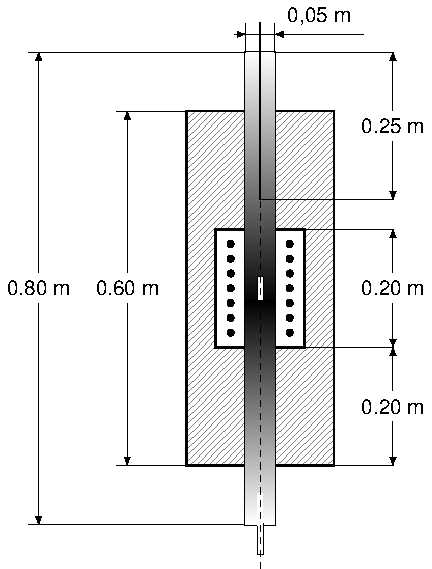
\includegraphics[width=6.5cm]{figures/ch-03-reacteur_pa}
  }\hfill
  \subfloat[\label{fig:reacteur_bp}Réacteur à basse pression.]{
    \raisebox{20mm}{
      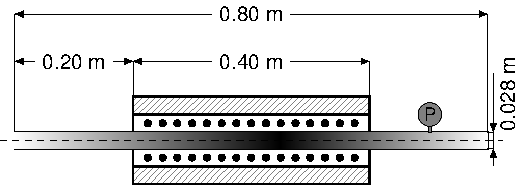
\includegraphics[width=8.5cm]{figures/ch-03-reacteur_bp}}
  }

  \caption{\label{fig:experimental_system}Schémas des réacteurs employés pour les traitements thermochimiques et le suivi de la décomposition des précurseurs.}
\end{figure}

\subsection{Réacteur à la pression atmosphérique}
\label{sec:reacteur_pa}

Les études de traitements thermochimiques ont été réalisées dans un réacteur tubulaire en alumine présentant un rapport surface-volume $\nicefrac{S}{V}=\SI{0,8}{\per\centi\metre}$ et un diamètre de \SI{50}{\milli\metre} schématisé Figure~\ref{fig:reacteur_pa}. L'enceinte de traitement en \ch{Al2O3} est considérée inerte, \textit{i.e.} les transformations chimiques des gaz précurseurs sont produites uniquement en phase homogène ou sur les surfaces des pièces traitées.  Pour assurer l'homogénéité en composition des gaz utilisés pour les traitements thermochimiques, un système d'alimentation de gaz permet le mélange des précurseurs dans un volume de ballast d'environ \SI{1000}{\cubic\centi\metre} avant introduction dans la zone de traitement du réacteur. L'injection des gaz se fait par un tuyau en alumine d'un diamètre interne de \SI{2}{\milli\metre} entrant par la partie supérieure du réacteur et injectant les gaz à \SI{100}{\milli\metre} de la partie supérieure de l'échantillon. Ceci permet d'assurer, pour les débits typiquement utilisés dans ce réacteur, de l'ordre de \SIrange{500}{1000}{\sccm}, la dissipation du jet de gaz produit par l'injecteur et un écoulement laminaire autour de la pièce traitée. Le chauffage est assuré par des résistances électriques placées autour de la zone centrale du tube réacteur sur une longueur de \SI{0,2}{\metre}, produisant une région de température constante d'environ \SI{80}{\milli\metre} et permettant des cycles thermiques jusqu'à \SI{1373}{\kelvin}. Cette zone est représentée sur la Figure~\ref{fig:experimental_system} par un gradient de gris, le rectangle central représentant la position de l'échantillon. Compte tenu de la longueur de cette région, pour assurer un traitement homogène des pièces, les échantillons ne doivent pas dépasser environ \SI{50}{\milli\metre} dans la direction de l'axe du réacteur. Par conséquent, des échantillons ayant des dimensions de \SI{40 x 14 x 4} {\milli\metre} ont été découpés dans des barres forgées des deux matériaux étudiés et polis au papier abrasif jusqu'à une granulométrie de \SI{14}{\micro\metre} avant traitement. Pour les suivis de prise de masse avec la thermobalance, chaque échantillon de longueur \SI{40}{\milli\metre} a été découpé en deux en raison de la limite de masse imposée par la thermobalance, conduisant à des pièces ayant pour dimensions \SI{20 x 14 x 4}{\milli\metre}. 

La caractérisation des produits à la sortie du réacteur est faite par un équipement de chromatographie gazeuse Carlo Erba Instruments modèle GC6000 Vega Series 2. Le système de chromatographie est équipé d'un détecteur à ionisation par flamme et d'un autre par conductivité thermique (Annexe~\ref{an:caracterisation_atmospheres}). La thermobalance couplée au système n'est pas représentée et se trouve à la verticale du réacteur. Une description détaillée de la thermobalance employée ici et de la technique de thermogravimétrie est fournie par \citet{Jaoul2004}. Un hygromètre Dewpro MMY 245 est aussi disponible pour la mesure de la température du point de rosée des atmosphères de cémentation.

\subsection{Réacteur à basse pression}
\label{sec:reacteur_bp}

\begin{figure}[!b]
  \centering\resizebox{0.6\textwidth}{!}{
    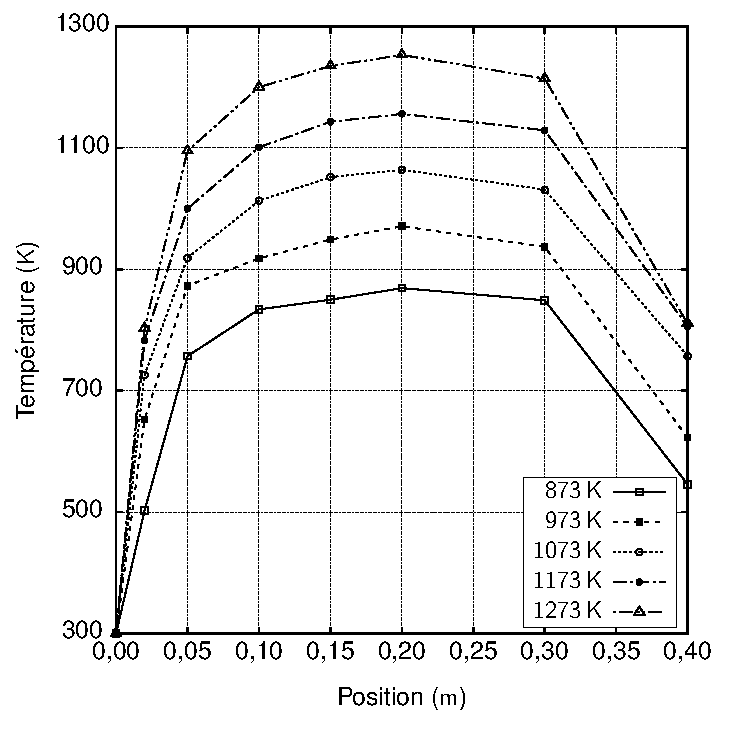
\includegraphics{figures/ch-03-reactor_bp_temperature}}
  
  \caption{\label{fig:temperature_profiles_bp}Profils de température dans la zone chaude du réacteur dans les expériences à basse pression (Figure~\ref{fig:reacteur_bp}) en fonction de la coordonnée de l'axe du réacteur mesurée à partir de l'entrée dans la zone de contrôle pour des températures de consigne entre \SIrange{873}{1273}{\kelvin}.}
\end{figure} 

Le système employé pour les études à basse pression est assez similaire de celui employé à la pression atmosphérique et le contrôle de son alimentation est réalisé par le même système et donc le même volume de ballast pour assurer l'homogénéité des gaz à l'entrée. L'alimentation des gaz est faite par la gauche (Figure~\ref{fig:reacteur_bp}), les systèmes de mesure de pression, de pompage et de caractérisation étant placés à droite. Le contrôle de température est opéré sur une longueur de \SI{0,4}{\metre} par des résistances disposées régulièrement, ce qui conduit aux profils présentés Figure~\ref{fig:temperature_profiles_bp}. Ces profils mesurés sont utilisés pour l'intégration des mécanismes cinétiques dans le Chapitre~\ref{ch:modelisation_cinetique}. Un tube en quartz présentant un rapport surface-volume $\nicefrac{S}{V}=\SI{1,4}{\per\centi\metre}$ et un diamètre de \SI{28}{\milli\metre} est utilisé comme enceinte de réacteur. Le système de chromatographie avec prélèvement à basse pression placé à la sortie de ce réacteur est décrit Section~\ref{sec:chromatographie_bp}.

\section{Caractérisation des réacteurs et des atmosphères}
\label{sec:caracterization_gaz}

\subsection{Dynamique du réacteur utilisé à la pression atmosphérique}
\label{sec:dynamique_experimentale}

Les fondements théoriques présentés à la Section~\ref{sec:dynamique} ont été utilisés pour l'évaluation du comportement dynamique du réacteur fonctionnant à la pression atmosphérique (Figure~\ref{fig:reacteur_pa}). Les mesures de distribution de temps de séjour $E(t_{s})$ ont été faites par le suivi de la réponse en tension d'un détecteur à ionisation par flamme en fonction du temps après injection d'un volume de \SI{10}{\cubic\centi\metre} de \ch{CH4} à l'entrée du réacteur. L'injection a lieu dans un intervalle de temps très court par rapport au temps de séjour estimé \textendash{} en considérant un débit de \SI{500}{\sccm} \textendash{} de l'ordre de \SI{100}{\second} pour un réacteur piston avec les dimensions du réacteur employé et de \SI{500}{\second} si l'on suppose un comportement de réacteur parfaitement agité. Étant donnée la faible quantité de méthane injectée, sa décomposition homogène n'est pas favorisée par la loi d'action de masse, ce qui rend possible l'évaluation de la fonction $E(t_{s})$. De plus, le \ch{CH4} est le composé le plus stable de la série des hydrocarbures aliphatiques. La détermination de la distribution de temps de séjour a été établie pour des débits de \SIlist{250;500;1000}{\sccm} à une température de \SI{1173}{\kelvin} en utilisant \ch{N2}  comme gaz porteur en l'absence d'un échantillon métallique à l'intérieur du réacteur.

Deux acquisitions ont été effectuées pour chaque condition. Ces essais ont été répétés avec une éprouvette métallique de dimensions \SI{40 x 14 x 4}{\milli\metre} placée à \SI{100}{\milli\metre} de l'injecteur de gaz dans l'axe du réacteur, les autres conditions restant inchangées. La face de \SI{14 x 4}{\milli\metre} était tournée vers le jet de gaz dans cette expérience. Un essai additionnel à \SI{1023}{\kelvin} avec un débit de \SI{500}{\sccm} a aussi été réalisé avec le four d'abord vide puis chargé. Le Tableau~\ref{tab:temps_caracteristics} rassemble les temps caractéristiques identifiés: $t_{\infty}$, le temps de disparition d'une espèce injecté par un pulse, $t_{m}$, le temps moyen de séjour et $\sigma$, le moment d'ordre un de la distribution de temps de séjour.

\begin{table}[!hb]
  \caption{\label{tab:temps_caracteristics}Temps caractéristiques du réacteur opéré à la pression atmosphérique en fonction des paramètres chargement, température et débit pour des mélanges dilués en \ch{N2} et nombre de Bodenstein associé.}
  
  \centering{}\footnotesize{}
  \begin{tabular}{\$c^c^c^c^c^c^c}
    \toprule[2pt]  
    \rowstyle{\bfseries}
    Condition 
    & Température $(\si{\kelvin})$ 
    & Débit $(\si{\cubic\centi\metre\per\minute})$
    & $t_{\infty}(\si{\second})$ 
    & $t_{m}(\si{\second})$
    & $\sigma(\si{\second})$
    & $Bo$
    \tabularnewline
    \midrule[2pt]  
    Non-chargé & 1023 & 500  & 657 & 250 & 112 & 6,5  \tabularnewline[6pt]
    Non-chargé & 1173 & 500  & 533 & 217 & 98  & 6,7  \tabularnewline[6pt]
    Non-chargé & 1173 & 1000 & 343 & 136 & 61  & 7,0  \tabularnewline[6pt]
    Chargé     & 1023 & 500  & 633 & 254 & 109 & 6,8  \tabularnewline[6pt]
    Chargé     & 1173 & 500  & 611 & 241 & 103 & 6,9  \tabularnewline[6pt]
    Chargé     & 1173 & 1000 & 361 & 127 & 62  & 5,9  \tabularnewline%
    \bottomrule
  \end{tabular}
\end{table}

Avant de procéder à l'analyse des résultats, quelques remarques préliminaires sont nécessaires. En supposant le réacteur à la température ambiante, on peut estimer que le délai entre l'injection du pulse de méthane et l'arrivée à la sortie du réacteur (Figure~\ref{fig:reacteur_pa}) est de l'ordre de \SI{100}{\second} pour un débit de \SI{500}{\cubic\centi\metre\per\minute} et de \SI{50}{\second} pour \SI{1000}{\cubic\centi\metre\per\minute}.  Si l'on considère une zone homogène de \SI{80}{\milli\metre} à la température de traitement $T_{r}$ (Section \ref{sec:experimental_system}) suivie d'un gradient de température décroissant jusqu'à l'ambiante à la sortie du réacteur, l'accélération produite par l'expansion du gaz devrait réduire ce temps par un facteur de l'ordre de 2,0. Cette réduction doit être plus faible, étant donnée l'augmentation de la viscosité du gaz porteur de \SIrange{17,5}{46,7}{\micro\pascal\second} entre \SIrange{298}{1173}{\kelvin}~\cite{Lienhard2008}. Par conséquent, le délai requis pour permettre l'arrivée du gaz au détecteur (Figure~\ref{fig:residence_time_distribution_raw}) est raisonnable puisqu'il n'est pas limité par le transport dans le tuyau qui conduit au détecteur.

\begin{figure}[h]
  \centering
  \subfloat[Réacteur non-chargé.]{
    \centering\resizebox{0.48\textwidth}{!}{
      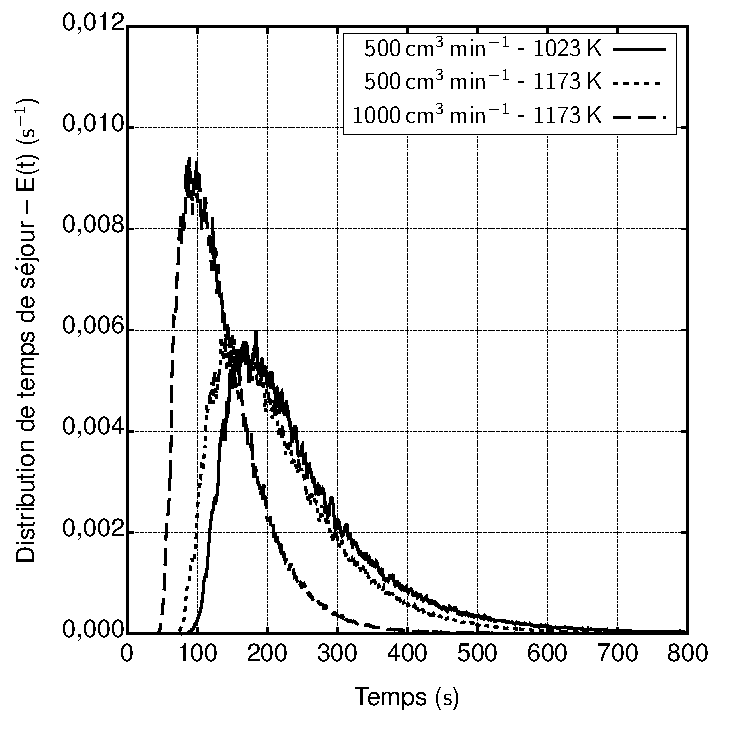
\includegraphics{figures/ch-03-rtd_raw_unloaded}}
  }\hfill
  \subfloat[Réacteur chargé.]{
    \centering\resizebox{0.48\textwidth}{!}{
      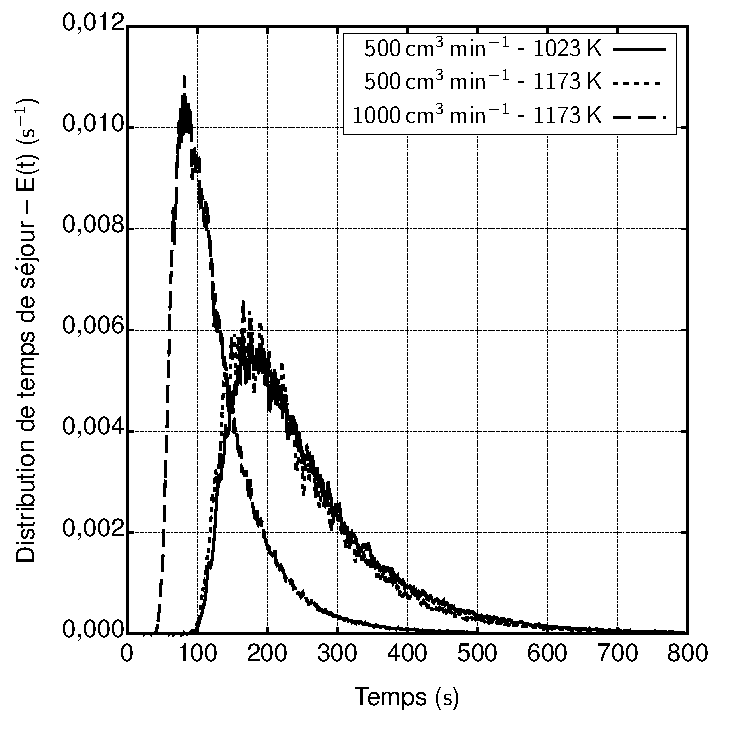
\includegraphics{figures/ch-03-rtd_raw_loaded}}
  }
  
  \caption{\label{fig:residence_time_distribution_raw}Densité de probabilité des distributions du temps de séjour non-normalisées en fonction du temps pour différentes conditions de débit et de température.}
\end{figure}

L'augmentation du débit diminue le temps de séjour moyen $t_{m}$ et réduit aussi la largeur $\sigma$ du pic de la densité de probabilité $E(t_{s})$, ce que l'on vérifie dans le comportement de la grandeur $\sigma$, le moment d'ordre 2 de la distribution, ce qui va à l'encontre des hypothèses définissant des réacteurs du type piston. La Figure~\ref{fig:residence_time_distribution_raw} met en évidence ce comportement du réacteur en fonction des différents débits employés avec et en l'absence d'un échantillon métallique. L'allure de ces courbes se rapproche du comportement d'un réacteur tubulaire laminaire, pour lequel un délai sur l'arrivée des espèces à la sortie produit une montée en intensité assez prononcée \textendash{} composante du comportement de type piston \textendash{} suivie d'une décroissance d'allure exponentielle \textemdash{} composante du comportement de type réacteur agité. À une température donnée, ce comportement est plus évident pour des débits plus élevés \textemdash{} le gaz est contraint de traverser le
réacteur sur une durée plus courte.

Si l'on compare les intégrales normalisées des courbes de la Figure~\ref{fig:residence_time_distribution_raw} tracées en fonction du temps réduit (Figure~\ref{fig:residence_time_distribution_integrated}) avec le comportement théorique (Figure~\ref{fig:types_de_reacteur}), on observe que le réacteur adopte un comportement approximativement du type laminaire. Les conditions expérimentales employées conduisent à des nombres de Reynolds de l'ordre de l'unité à la pression atmosphérique. Les traitements sous vide mènent à des valeurs beaucoup plus faibles et donc l'écoulement doit aussi être laminaire. Le nombre de Knudsen estimé Section~\ref{sec:cinetique} assure un comportement du type visqueux dans les deux limites de pression étudiées. Les courbes intégrées et normalisées (Figure~\ref{fig:residence_time_distribution_integrated})  montrent~\cite{Fogler1999} que dans la plage de débits étudiée, le réacteur conserve le même type de comportement. Le chargement du réacteur à la température de traitement avec des pièces métalliques agit quant à lui dans le sens d'une faible augmentation du temps de séjour  moyen. Lorsque l'effet du chargement avec des échantillons de même taille que ceux qui sont utilisés pour les études métallurgiques ne produit pas de changement important de $t_{m}$, on se contente alors de réaliser les études expérimentales sur la pyrolyse de l'acétylène et de l'ammoniac sans échantillon. Cela permet aussi de séparer les effets de catalyse sur les surfaces métalliques des phénomènes ayant lieu dans le gaz ou sur les parois du réacteur.

\begin{figure}[h]
  \centering
  \subfloat[Réacteur non-chargé.]{
    \centering\resizebox{0.48\textwidth}{!}{
    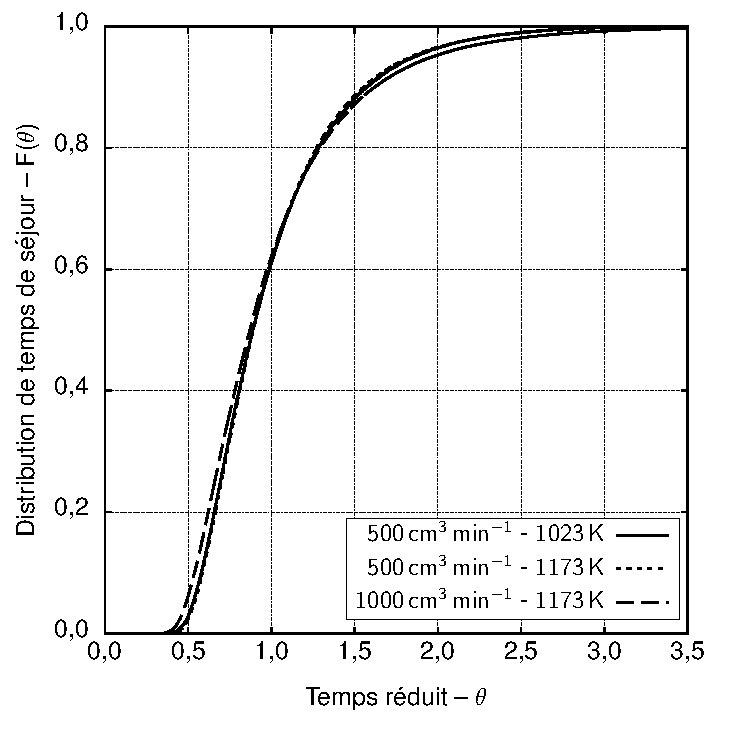
\includegraphics{figures/ch-03-rtd_unloaded}}
  }\hfill
  \subfloat[Réacteur chargé.]{
    \centering\resizebox{0.48\textwidth}{!}{
    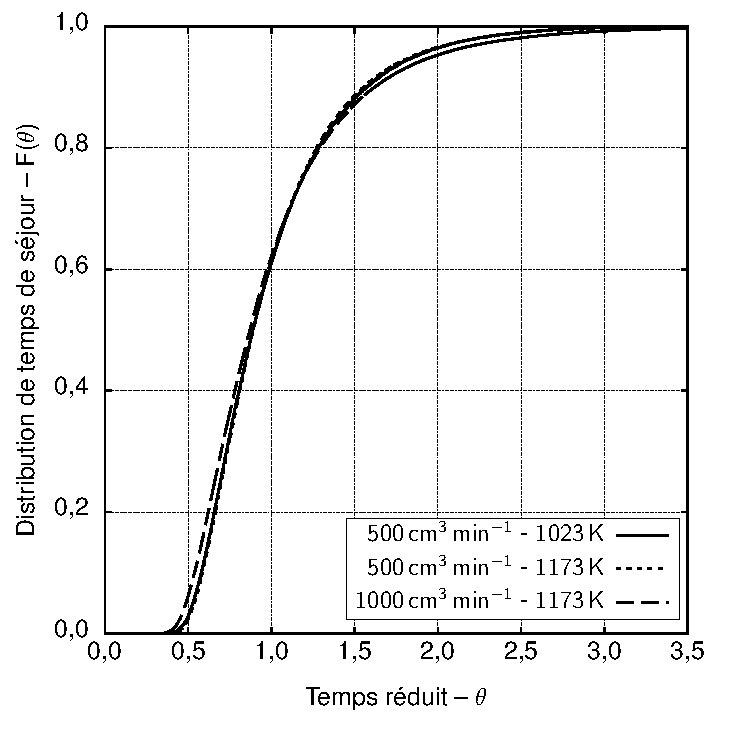
\includegraphics{figures/ch-03-rtd_loaded}}
  }

  \caption{\label{fig:residence_time_distribution_integrated}Distributions du temps de séjour intégrées et normalisées en fonction du temps réduit $\theta$. Les courbes sont identifiées par les conditions de débit et de température.}
\end{figure}

Le comportement de mélange des nouveaux éléments de volume arrivant dans l'enceinte du réacteur peut être caractérisé par les nombres de Bodenstein ou de Peclet axial~\cite{Becker1998177,Fogler1999}.  Les définitions de ces nombres sont présentées Équation~\ref{eq:bodenstein_peclet}, où $D$ désigne le coefficient de diffusion moléculaire, $d$ le diamètre du tube, $L$ sa longueur et $\bar{\nu}$ la vitesse moyenne. Une valeur élevée ($Bo{}\geq{}50$) implique un comportement de ségrégation \textendash{} les nouveaux volumes rentrant dans le réacteur ne sont pas dilués dans le contenu de l'enceinte~\cite{Becker1998177} \textendash{} tandis qu'un réacteur agité possède un nombre de Bodenstein réduit. Ce critère n'est valable que pour des ratios $\nicefrac{L}{d}\geq40$ et son utilisation directe produit une incertitude importante. Dans ce cas, l'ajustement des distributions expérimentales au moyen de l'Équation~\ref{eq:rtd_bodenstein} conduit à des résultats plus fiables~\citep{Becker1998177}.

\begin{equation}
  Pe_{ax}=\frac{192D}{\bar{\nu}d}\quad\quad\quad 
  Bo=Pe_{ax}\frac{L}{d}
  \label{eq:bodenstein_peclet}
\end{equation}

\begin{equation}
  E(\theta)=\frac{1}{2}\sqrt{\frac{Bo}{\pi\theta}}
    \biggr[\exp\biggr(\frac{(1-\theta)^{2}Bo}{4\theta}\biggr)\biggr]^{-1}
  \label{eq:rtd_bodenstein}
\end{equation}

Les valeurs ainsi obtenues pour le nombre de Bodenstein (Tableau~\ref{tab:temps_caracteristics}) montrent que le chargement et/ou l'augmentation du débit conduisent à l'augmentation de l'effet de mélange dans le réacteur. Pour des valeurs de l'ordre de 5, le comportement de mélange ne peut pas être considéré comme étant ségrégé.  Ces estimations ne sont valables que pour le méthane, mais l'ordre de grandeur et le type de comportement restent inchangés pour d'autres espèces, en raison de la proximité des valeurs des coefficients de diffusion des hydrocarbures légers et de celles des dérivés de l'ammoniac dans les gaz utilisés~\footnote{Pour leurs sections de collision, voir \citet{Bird}, par exemple.}.  
Alors que la valeur de $t_{m}$ est associée aux taux d'avancement des réactions globales de décomposition des gaz précurseurs et donc au comportement du réacteur à l'état stationnaire, c'est la valeur de $t_{\infty}$ qu'il convient de considérer pour connaitre le temps nécessaire au renouvellement de l'atmosphère \textemdash{} ici déterminée pour une valeur de $F(t_{\infty})=0,99$. Cette valeur de $t_{\infty}$ représente donc le temps minimal pour démarrer le suivi de la pyrolyse des atmosphères à l'état stationnaire et aussi le temps nécessaire pour atteindre des enrichissements à concentration constante pour les atmosphères à l'équilibre thermodynamique, comme dans le cas de la cémentation à partir de mélanges \ch{CO-H2}.

\subsection{Chromatographie gazeuse à basse pression}
\label{sec:chromatographie_bp}

La mise au point des traitements thermochimiques demande la connaissance préalable de la cinétique de décomposition des précurseurs pour l'enrichissement des matériaux dans la gamme de pressions étudiée. Pour cela, cette étude comprend des mesures par chromatographie gazeuse des produits issus de la décomposition de l'ammoniac et de l'acétylène. Bien que la chromatographie gazeuse à la pression atmosphérique soit une technique bien connue et employée dans la caractérisation des atmosphères gazeuses, son emploi sous pression réduite n'est pas simple. Cette section décrit la méthode employée pour réaliser l'acquistion des chromatogrammes à basse pression ainsi que les limitations qui doivent être prises en compte dans l'analyse des résultats.

L'acquisition des données à basse pression se fait par un équipement Perkins Elmer modèle Clarus 580 équipé d'une colonne pour la séparation primaire des composants qui sont ensuite divisés dans une colonne Molsieve 5A pour la séparation des composants de la bande atmosphérique (\ch{N2}, \ch{O2}, \ch{CH4}, etc.) et dans une colonne Poraplot U pour l'identification des hydrocarbures et de l'ammoniac. La détection de ces produits se fait par un détecteur du type TCD. Bien qu'il s'agisse d'un système conventionnel de chromatographie gazeuse, le prélèvement de l'échantillon pour l'injection dans les colonnes se fait d'une façon particulière. Le système mis en place est connecté à une des sorties du réacteur employé dans l'étude, laquelle est soumise à un pompage intermittent vers le système de prélèvement à basse pression. L'appareil est composé d'une série de vannes qui permettent le remplissage d'un ballon en élastomère par les produits prélevés à la sortie du réacteur, ballon qui fait office d'enceinte tampon. Après le remplissage du ballon, les gaz ainsi prélevés sont comprimés à la pression atmosphérique puis injectés dans la boucle de prélèvement de l'équipement de chromatographie. La Figure~\ref{fig:systeme_bp} présente un schéma du système de prélèvement, où \og{}$B$\fg{} désigne le ballon d'échantillonnage et \og{}$P$\fg{} la pompe à vide. La séquence d'opérations automatisée du système est fournie Annexe~\ref{an:caracterisation_atmospheres}. %et certains détails complémentaires.

\begin{figure}[h]
  \centering\resizebox{0.6\textwidth}{!}{
    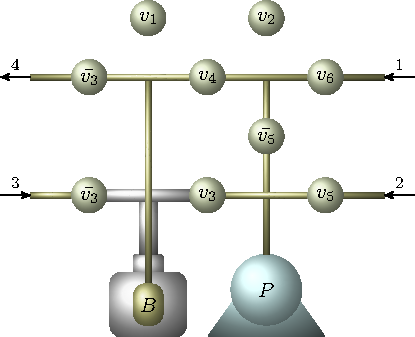
\includegraphics{figures/ch-03-schema_gcbp}}
  
  \caption{\label{fig:systeme_bp}Système de prélèvement à basse pression. Les flèches désignent: 1 -- le prélèvement du réacteur, 2 -- la sortie du système de chromatographie, 3 -- l'entrée d'air pour comprimer l'échantillon et 4 -- l'injection du système de chromatographie.}
\end{figure}

Ce système permet une acquisition reproductible des chromatogrammes au--delà de \SI{30}{\milli\bar} avec l'accumulateur \og{}$B$\fg{} utilisé. Pour travailler à plus faible pression, un accumulateur de volume supérieur est requis. Bien que l'acquisition soit reproductible, elle reste faiblement dépendante de la pression totale du système, impliquant le besoin d'un étalonnage pour chaque pression utilisée dans l'étude. Au moment du détournement du gaz vers l'accumulateur, le réacteur est soumis à des variations momentanées de pression qui sont contrôlées manuellement pendant l'acquisition de l'échantillon. Ces oscillations conduisent à des erreurs relatives de mesure qui peuvent atteindre 10\% entre \SIrange{30}{100}{\milli\bar}. %De plus, étant donné que de faibles admissions des gaz de l'atmosphère dans le réacteur au cours de cette étape, l'étalonnage est limité en précision et dépendant des ce fuites qui sont dépendant naturellement de la pression d'opération.

\section{Cémentation à partir des mélanges \ch{CO-H2}}
\label{sec:classical_carburizing}

Afin d'assurer une saturation de la surface en carbone pour les traitements de cémentation à partir des mélanges gazeux, une étude thermodynamique de l'équilibre gaz--solide a été menée pour chaque alliage. Cela a été fait de manière à employer une méthode basée sur la mesure de la température du point de rosée $T_{r}$ des effluents du réacteur. Le calcul de $T_{r}$ a été réalisé en considérant l'atmosphère de cémentation (Tableau~\ref{tab:treatment_atmospheres}). Les paramètres de \citet{Gunnarson1967} des alliages étudiés sont calculés, conduisant à $Q=1,1$ pour l'alliage 16NiCrMo13 et $Q=0,9$ pour la nuance 23MnCrMo5. Il existe une plus forte affinité avec le carbone pour l'alliage 23MnCrMo5 \textendash{} visible sur la Figure~\ref{fig:dew_point} en fixant une valeur de $T_{r}$: la fraction massique en carbone en équilibre entre le matériau et l'atmosphère est plus élevée pour cette nuance que pour l'alliage 16NiCrMo13. La Figure~\ref{fig:dew_point} compare également les résultats du calcul de $T_{r}$ selon la méthode classique présentée Section~\ref{sec:controle_cementation} à ceux des simulations effectuées avec Thermo-Calc~\cite{Andersson2002,Borgenstam2000} \textendash{} les températures $T_{r}$ à la saturation en carbone dans les alliages diffèrent de moins de \SI{1}{\kelvin} et l'écart entre les méthodes ne dépasse pas \SI{3}{\kelvin} en dessous de cette limite. La divergence des courbes que l'on observe au--delà de la limite de saturation des alliages s'explique par le fait que l'Équation~\ref{eq:ellis_carbone} ne considère pas de transitions de phase. Il est important que la température de point de rosée pendant les traitements ne soit pas inférieure à celle conduisant à la saturation, ce qui peut entrainer une précipitation importante de cémentite. L'Annexe~\ref{an:dew-point} présente les détails de ces simulations.

\begin{table}[h]
  \caption{\label{tab:treatment_atmospheres}Atmosphères pour les étapes de cémentation et de nitruration des traitements réalisés à la pression atmosphérique.}
  
  \centering{}\footnotesize{}%
  \resizebox{\textwidth}{!}{
    \begin{tabular}{\$c^c^c^c^c^c^c}
      \cmidrule[2pt]{1-3}  \cmidrule[2pt]{5-7}  
      \multicolumn{3}{c}{\bfseries Cémentation} 
      & & 
      \multicolumn{3}{c}{\bfseries Nitruration}
      \tabularnewline
      \cmidrule[2pt]{1-3}  \cmidrule[2pt]{5-7}  
      {0,20 \ch{CO}} & {0,40 \ch{H2}} & {0,40 \ch{N2}} 
      & & 
      {0,04 \ch{NH3}} & {0,72 \ch{H2}} & {0,24 \ch{N2}}
      \tabularnewline[6pt]
      %
      {\SI{100}{\sccm}} & {\SI{200}{\sccm}} & {\SI{200}{\sccm}} 
      & & 
      {\SI{15}{\sccm}} & {\SI{300}{\sccm}} & {\SI{100}{\sccm}}
      \tabularnewline
      \cmidrule{1-3}  \cmidrule{5-7} 
    \end{tabular}
  }
\end{table}

\begin{figure}[!ht]
  \centering
  \subfloat[Alliage 16NiCrMo13.]{
    \centering\resizebox{0.48\textwidth}{!}{
    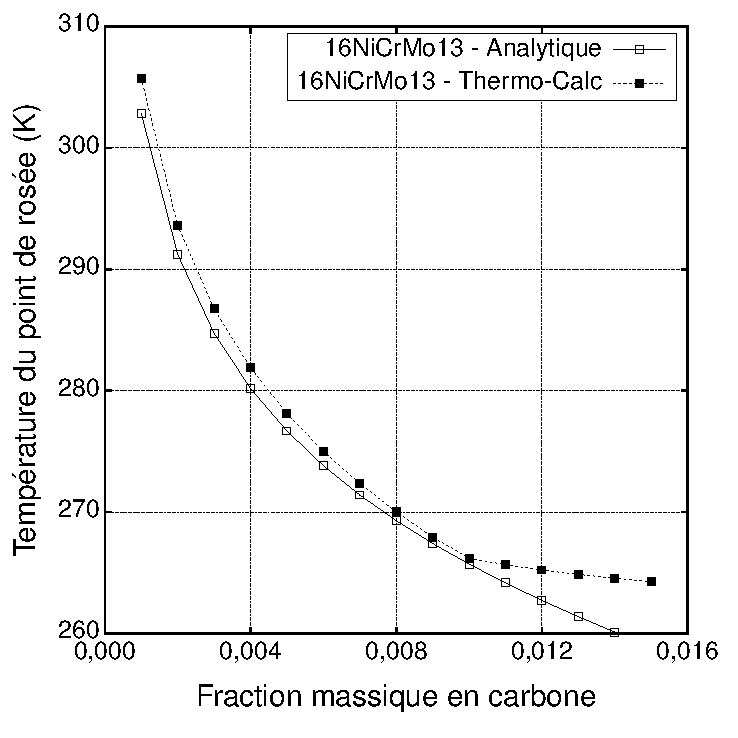
\includegraphics{figures/ch-03-dew_point_aero}}
  }\hfill
  \subfloat[Alliage 23MnCrMo5.]{
    \centering\resizebox{0.48\textwidth}{!}{
    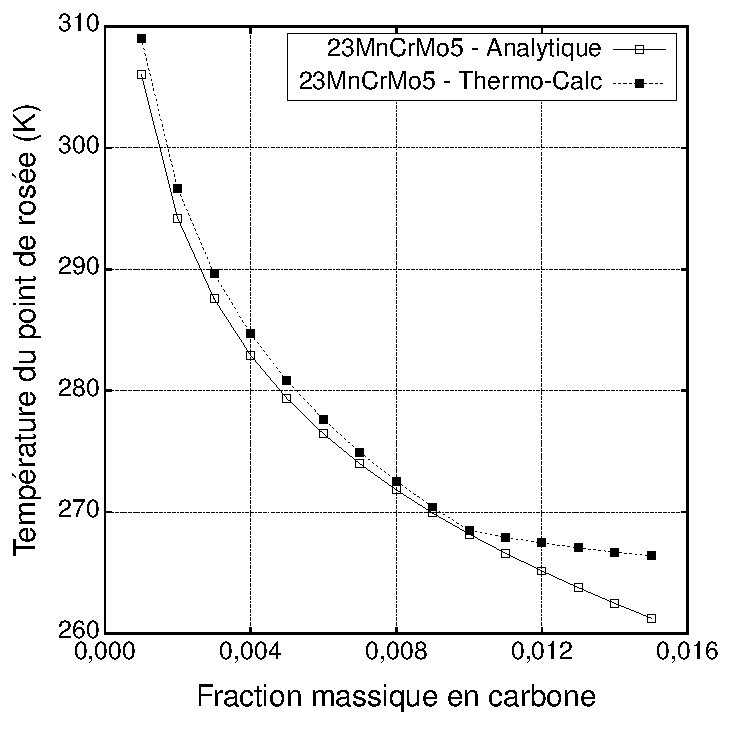
\includegraphics{figures/ch-03-dew_point_auto}}
  }

  \caption{\label{fig:dew_point}Température du point de rosée en fonction de la fraction massique en carbone à l'équilibre avec l'atmosphère de traitement.}
\end{figure}

\section{Procédés à partir des hydrocarbures}
\label{sec:pyrolyse_acetylene}

L'étude de la pyrolyse de l'acétylène, précurseur du carbone pour l'étape de cémentation, s'est faite par chromatographie en phase gazeuse. Les mesures effectuées visent à fournir des indications sur les espèces présentes dans le réacteur pour le transfert de matière vers le solide, sur les mécanismes de surface régissant les traitements évalués et sur la validité des mécanismes développés. L'étude des réactions de surface s'opère généralement par une analyse différentielle des produits obtenus en l'absence et en présence d'un échantillon. Pour cela, on suppose que la réactivité des parois en alumine du réacteur est négligeable par rapport aux effets induits par les surfaces des éprouvettes métalliques.  On commence donc par étudier le réacteur non-chargé. Les paramètres de contrôle pris en compte pour l'étude sont le débit total, le débit du précurseur étudié et la température. % dans la zone de contrôle du réacteur.

\subsection{Pyrolyse à la pression atmosphérique}

Les expériences à la pression atmosphérique ont été réalisées en employant \ch{N2} comme gaz porteur et ont permis le suivi de la pyrolyse de l'acétylène dans la plage de température allant de \SIrange{873}{1223}{\kelvin}. Afin d'établir une pression partielle de \ch{C2H2} de l'ordre de \SI{20}{\hecto\pascal}, pression de référence dans cette étude pour les traitements à basse pression, un mélange contenant \ch{N2 - 0,02 C2H2} en fraction volumique a été employé, et ce pour des débits de \SIlist{500;1000}{\cubic\centi\metre\per\minute}. Ces conditions sont résumées Tableau~\ref{tab:pyrolysis-conditions-pa}. La caractérisation de cette atmosphère en sortie du réacteur a permis la quantification des hydrocarbures légers \ch{CH4}, \ch{C2H2} et \ch{C2H4} et \ch{H2} à l'aide du détecteur FID du chromatographe. L'acquisition des données s'est faite toutes les \SI{20}{\minute} pour les hydrocarbures et toutes les \SI{4}{\minute} pour \ch{H2}, qui est mesuré par le détecteur TCD. 

\begin{table}[h]
  \caption{\label{tab:pyrolysis-conditions-pa}Conditions expérimentales pour l'étude de la pyrolyse du \ch{C2H2} à pression atmosphérique dans le réacteur présenté Figure~\ref{fig:reacteur_pa}.}
  
  \resizebox{\textwidth}{!}{
  \footnotesize{}\centering{}
  \begin{tabular}{\$c^c^c^c^c}
    \toprule[2pt]
    \rowstyle{\bfseries}
    Température 
    & Débit 
    & Mélange 
    & Pression totale 
    & Pression \ch{C2H2}
    \tabularnewline
    \midrule[2pt]
    \SIrange{873}{1223}{\kelvin} 
    & \SIlist{500;1000}{\sccm}
    & \ch{N2 - 0,02 C2H2}
    & \SI{1000}{\hecto\pascal}
    & \SI{20}{\hecto\pascal}
    \tabularnewline
    \bottomrule
  \end{tabular}
  }
\end{table}

Les fractions molaires des espèces identifiées à l'état stationnaire sont présentées Figure~\ref{fig:acetylene_pyrolysis} en fonction de la température de la zone chaude du réacteur. On vérifie que même pour des temps de séjour supérieurs à \SI{100}{\second}, l'acétylène est l'hydrocarbure léger majoritaire. En dessous de \SI{900}{\kelvin} le craquage de \ch{C2H2} est négligeable par rapport à la concentration injectée dans le réacteur et l'étude se limite à des mesures au--dessus de \SI{873}{\kelvin}. On observe aussi le rôle du temps de séjour : à une température donnée, une augmentation du débit produit une plus faible conversion du gaz source en sous-produits, tel qu'on peut le mettre en évidence pour les températures de \SIrange{1023}{1223}{\kelvin} en comparant les fractions de \ch{C2H2} et \ch{H2}, et est équivalente à un décalage de \SI{50}{\kelvin} dans\textsl{} la zone chaude du réacteur. %Pour les distributions de temps de séjour de la Figure~\ref{fig:residence_time_distribution_raw}, cette augmentation de débit est équivalente à une décalage de \SI{50}{\kelvin} dans la température de la zone chaude du réacteur.

\begin{figure}[!ht]
  \centering
  \subfloat[Toutes les espèces.]{
    \centering\resizebox{0.98\textwidth}{!}{
      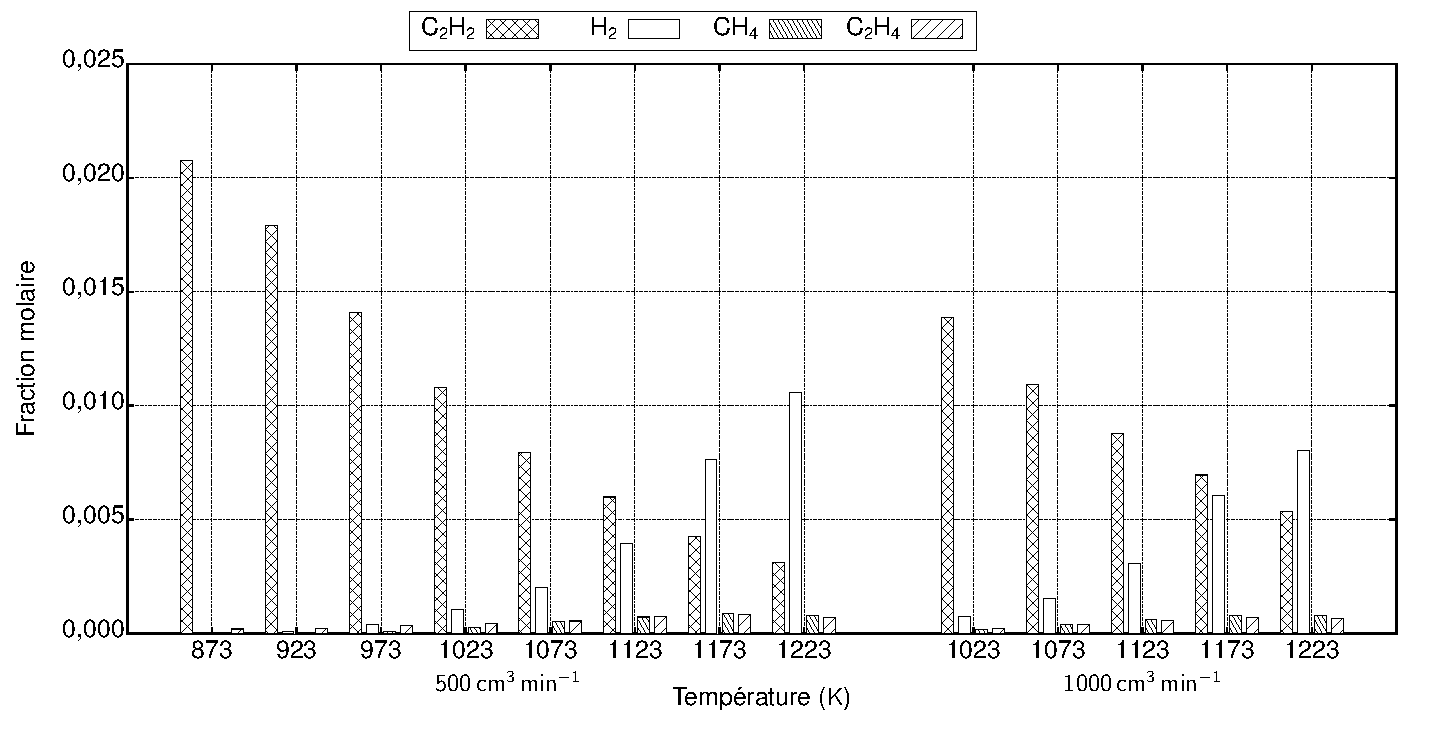
\includegraphics{figures/ch-03-decomposition_c2h2_all_pa}}
  }\\
  \subfloat[Espèces minoritaires.]{
    \centering\resizebox{0.98\textwidth}{!}{
      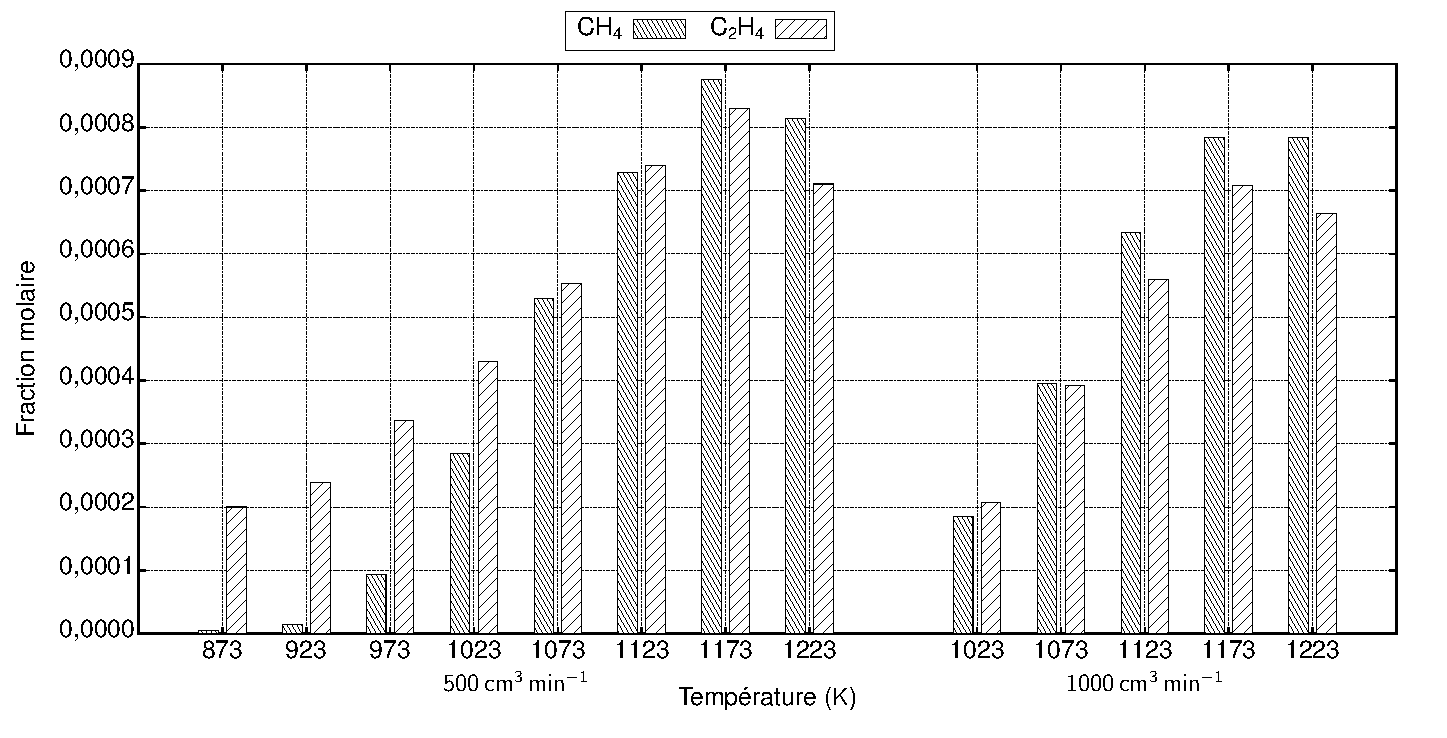
\includegraphics{figures/ch-03-reaction_byproducts_pa}}
  }
  
  \caption{\label{fig:acetylene_pyrolysis}Suivi des produits de pyrolyse de l'acétylène à la pression atmosphérique en fonction de la température de la zone chaude du réacteur. Les produits mesurés sont fonctions des interactions entre le gradient de température et la distribution $E(t_{s})$ pour les débits de \SIlist{500;1000}{\sccm}.}
\end{figure}

Selon les données du Tableau~\ref{tab:temps_caracteristics}, l'augmentation du débit de \SIrange{500}{1000}{\sccm} n'a pas seulement réduit le temps de séjour moyen à l'intérieur du four, mais a aussi diminué la largeur du pic de densité de probabilité, les deux effets combinés conduisant aux réponses mesurées. %Une autre manière de décrire ce comportement, consiste à dire que l'augmentation du débit diminue la valeur de $Bo$, ce qui favorise le comportement de mélange dans le réacteur et permet donc que le précurseur sorte plus tôt du réacteur. 
Il faut aussi tenir compte du fait que la pyrolyse se passe dans une zone comportant un gradient de température si bien que les produits analysés proviennent de différentes zones du réacteur. La réduction de la température de la zone chaude implique aussi l'augmentation du temps de séjour avec un élargissement du pic de la $E(t_{s})$.  Étant donné que les temps de séjour sont beaucoup plus longs que ceux employés par~\citet{Norinaga2005,Norinaga2007}, il en résulte que la décomposition de l'acétylène et la formation de \ch{CH4} et \ch{C2H4} sont beaucoup plus avancées. Ces résultats se rapprochent des observations faites par \citet{Graf2007} et \citet{Khan2008}.

Le bilan matière des espèces rapportées sur la Figure~\ref{fig:acetylene_pyrolysis} n'atteint pas l'unité: il est donc possible d'estimer la composition des espèces inconnues dans le système et la fraction qu'elles représentent. Tout d'abord, on calcule l'apport de chaque espèce mesurée $\phi$ à la fraction des atomes $i$ composant le système \textendash{} le carbone et l'hydrogène \textendash{} récupérés à la sortie. Cette contribution $\psi_{i,\phi}$ s'exprime selon $\psi_{i,\phi}=n_{i,\phi}\times x_{\phi}$, où $n_{i,\phi}$ désigne le nombre d'atomes de $i$ dans $\phi$ et $x_{\phi}$ la fraction molaire mesurée de cette espèce. La fraction d'atomes $i$ récupérée à la sortie par rapport à celle à l'entrée, que l'on notera $\Psi_{i}$, est définie par le rapport entre les sommes des $\psi_{i,\phi}$ à la sortie et à l'entrée du réacteur.  Pour le carbone et l'hydrogène, grâce aux données acquises, on peut écrire les Équations~\ref{eq:psi_c}~et~\ref{eq:psi_h}, respectivement, où les numérateurs sont des sommes pondérées des fractions molaires des produits à la sortie et les dénominateurs la fraction molaire du précurseur à l'entrée. L'hypothèse de débit volumique constant est raisonnable compte tenu de la dilution du mélange à l'entrée et du comportement de pyrolyse de l'acétylène~\cite{Norinaga2005}.

\begin{equation}
  \Psi_{\ch{C}}=\dfrac{1\times x_{\ch{CH4},s}+2\times x_{\ch{C2H2},s}+2\times x_{\ch{C2H4},s}+0\times x_{\ch{H2},s}}{2\times x_{\ch{C2H2},e}}
  \label{eq:psi_c}
\end{equation}

\begin{equation}
  \Psi_{\ch{H}}=\dfrac{4\times x_{\ch{CH4},s}+2\times x_{\ch{C2H2},s}+4\times x_{\ch{C2H4},s}+2\times x_{\ch{H2},s}}{2\times x_{\ch{C2H2},e}}
  \label{eq:psi_h}
\end{equation}

Indépendamment de cette approche, on vérifie Figure~\ref{fig:balance_molaire} que dans la plage de température typique de la cémentation/carbonitruration \textendash{} \SIrange{1173}{1223}{\kelvin} \textendash{} il reste moins de 30\% de carbone sous forme d'hydrocarbures légers pour tous les débits considérés.  Environ 70-80\% du carbone se trouve sous forme d'hydrocarbures plus lourds ou de suies non mesurées. Ces courbes permettent aussi d'identifier la fraction des atomes d'hydrogène présents dans des hydrocarbures non-mesurés. Contrairement au carbone, à haute température, la localisation de l'hydrogène dans des molécules est connue à environ 80\%. Dans tout le domaine de température balayé, la fraction d'hydrogène présente dans les hydrocarbures est inférieure à celle sous forme de \ch{H2}.

\begin{figure}[!ht]
  \centering
  \subfloat[\label{fig:bilan-atomique-pa}Bilan atomique.]{
    \centering\resizebox{0.98\textwidth}{!}{
      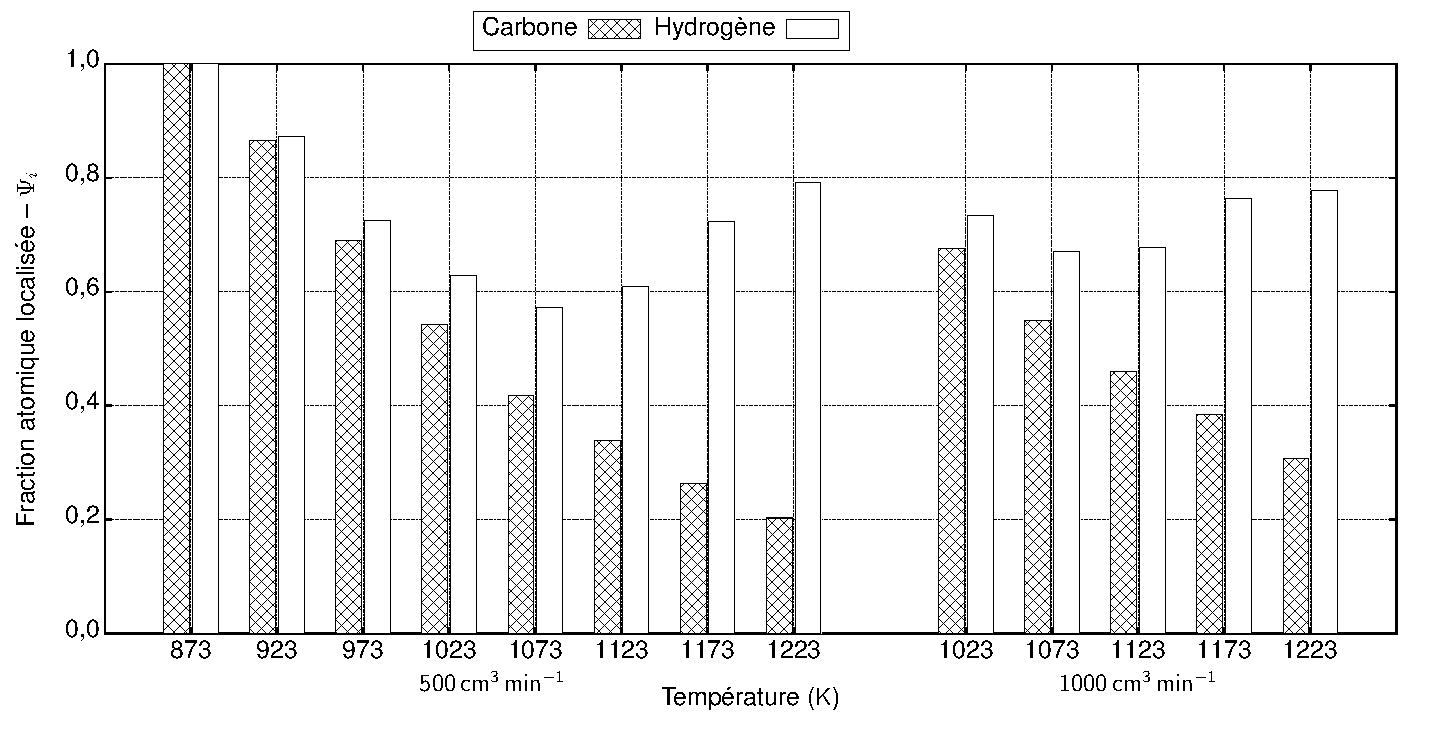
\includegraphics{figures/ch-03-balance_molaire}}
  }\\
  \subfloat[\label{fig:ration_ch}Rapport $\nicefrac{\ch{C}}{\ch{H}}$.]{
    \centering\resizebox{0.98\textwidth}{!}{
      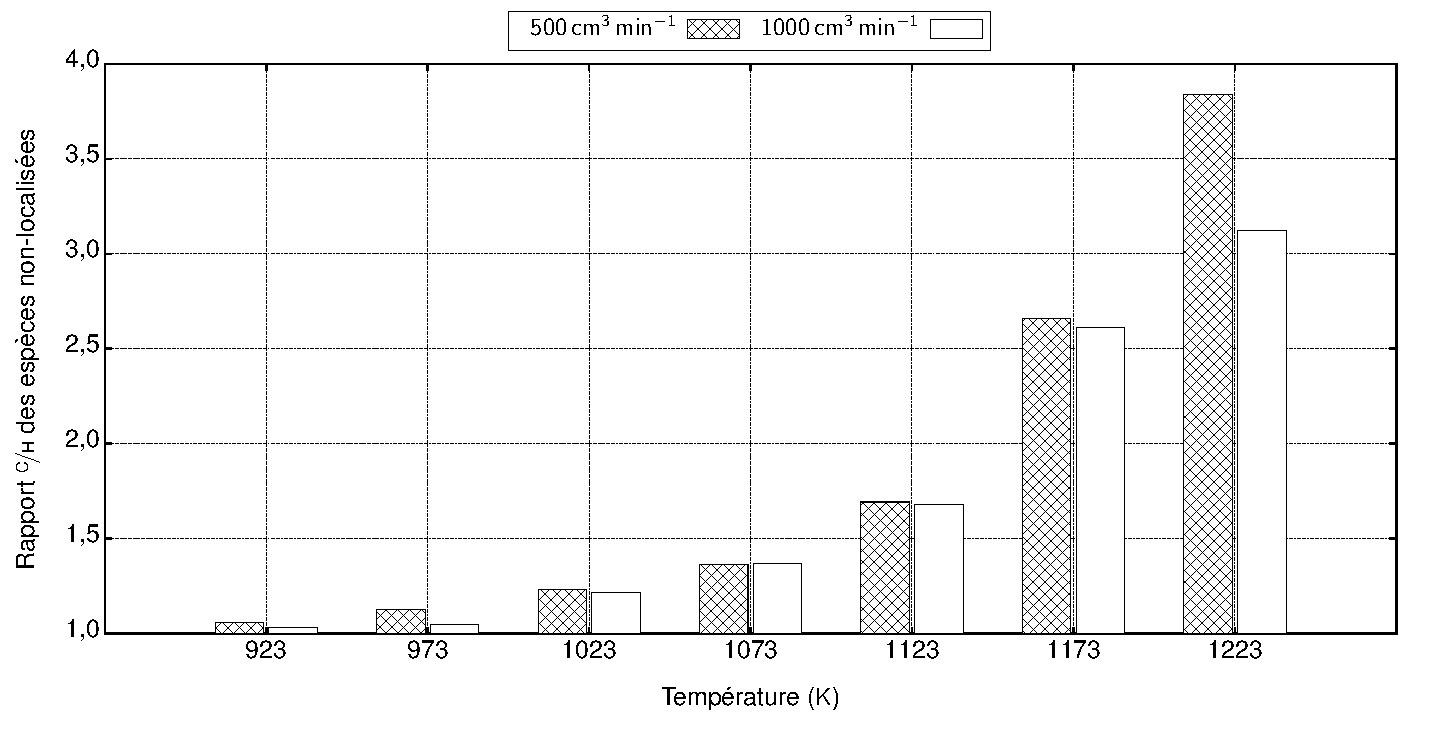
\includegraphics{figures/ch-03-ratio_carbon_hydrogen}}
  }

  \caption{\label{fig:balance_molaire}Bilan matière de la pyrolyse de l'acétylène à la pression atmosphérique réalisé à partir des données de la Figure~\ref{fig:acetylene_pyrolysis} et rapport  calculé entre le nombre d'atomes de carbone et d'hydrogène dans les espèces non-détectées.}
\end{figure}

On observe (Figure~\ref{fig:ration_ch}) que le rapport $\nicefrac{\ch{C}}{\ch{H}}$ des espèces inconnues augmente dans la plage de température étudiée, ce qui implique une réduction des saturations dans les hydrocarbures.  Par exemple, sur plus de 200 espèces présentes dans le mécanisme cinétique compilé par \citet{Norinaga2007}, à peine une dizaine d'entre elles possèdent un ratio $\nicefrac{\ch{C}}{\ch{H}}\geq2,0$, à savoir celles de la famille du coronène. La majorité des composants aromatiques légers se situe entre 1,0 et 2,0. Le benzo(a)pyrène, composant indésirable pour des raisons de santé, présente un rapport $\nicefrac{\ch{C}}{\ch{H}}=1,67$. Les ratios au-delà de 3,0 représentent des radicaux riches en carbone (\ch{C3H}, \ch{C6H}, etc.) ou des dépôts de suie issus de la pyrolyse.  Au--dessus de \SI{1123}{\kelvin} ce ratio croît rapidement, condition pour laquelle la pollution du four et la formation de dépôts est favorisée.

\subsection{Pyrolyse sous pression réduite}
\label{sec:pyrolyse_acetylene_bp}

La cinétique de pyrolyse de l'acétylène a été étudiée à basse pression en utilisant le réacteur décrit Section \ref{sec:reacteur_bp}. Ces expériences ont été réalisées dans la plage de pressions entre \SIrange{30}{100}{\hecto\pascal} en utilisant un mélange \ch{N2 - 0,36 C2H2} sous un débit de \SI{222}{\sccm} \textemdash{} Tableau~\ref{tab:pyrolysis-conditions-bp}. Les résultats de ces mesures se trouvent Figure~\ref{fig:pyrolyse_acetylene_bp}. L'étalonnage du système a été réalisé à la pression de \SI{50}{\milli\bar} et complété par des vérifications aux pressions limites utilisées dans l'expérience. Le système de compression permet un remplissage complet de la boucle de prélèvement du chromatographe à partir de \SI{30}{\milli\bar} et la calibration est indépendante de la pression. Cela n'empêche pas l'utilisation de ce système en dessous de \SI{30}{\milli\bar}, mais dans ce cas un étalonnage doit être réalisé pour chaque pression utilisée et les résultats sont beaucoup moins reproductibles en dessous de ce seuil d'opération. %~\footnote{En outre, du fait de la perturbation causée par le système de pompage pendant le prélèvement de l'échantillon, les résultats sont beaucoup moins reproductibles en dessous de ce seuil d'opération.}. %L'oxygène résiduel a été inclus dans le bilan matière en utilisant une correction de la courbe d'étalonnage du di-azote ce qui est possible en raison de leurs diffusivités thermiques assez proches~\footnote{Conductivité égale à \SI{38,8}{\milli\watt\per\metre\per\kelvin} pour \ch{N2} contre \SI{40,1}{\milli\watt\per\metre\per\kelvin} pour \ch{O2} à une température de \SI{500}{\kelvin}~\cite{Lienhard2008}, i.e. de l'ordre de celle du détecteur TCD.  Ces espèces présentent des capacités calorifiques de \SI{1055}{\joule\per\kilo\gram\per\kelvin} et \SI{972}{\joule\per\kilo\gram\per\kelvin}, ce qui conduit au rapport entre les diffusivités thermiques $\nicefrac{\alpha_{\ch{O2}}}{\alpha_{\ch{N2}}}=1,12$.}. Cela confirme la présence des traces de \ch{O2}, de l'ordre de \SI{1000}{ppm} dans la bouteille de \ch{N2} et permet l'identification jusqu'à 2\% du flux d'espèces provenant de l'atmosphère extérieure donnée des fuites de l'installation.

\begin{table}[h]
  \caption{\label{tab:pyrolysis-conditions-bp}Conditions expérimentales pour l'étude de la pyrolyse du \ch{C2H2} à basse pression dans le réacteur présenté Figure~\ref{fig:reacteur_bp}.}
  
  \footnotesize{}\centering{}
  \begin{tabular}{\$c^c^c^c^c}
    \toprule[2pt]
    \rowstyle{\bfseries}
    Température 
    & Débit 
    & Mélange 
    & Pression totale 
    & Pression \ch{C2H2}
    \tabularnewline
    \midrule[2pt]
    \SIrange{773}{1273}{\kelvin}
    & \SI{222}{\sccm}
    & \ch{N2 - 0,36 C2H2}
    & \SIrange{30}{100}{\hecto\pascal}
    & \SIrange{10,8}{36,0}{\hecto\pascal}
    \tabularnewline
    \bottomrule
  \end{tabular}
\end{table}

\begin{figure}[!ht]
  \centering
  \subfloat[\label{fig:acetylene_bp}Acétylène.]{
    \centering\resizebox{0.98\textwidth}{!}{
      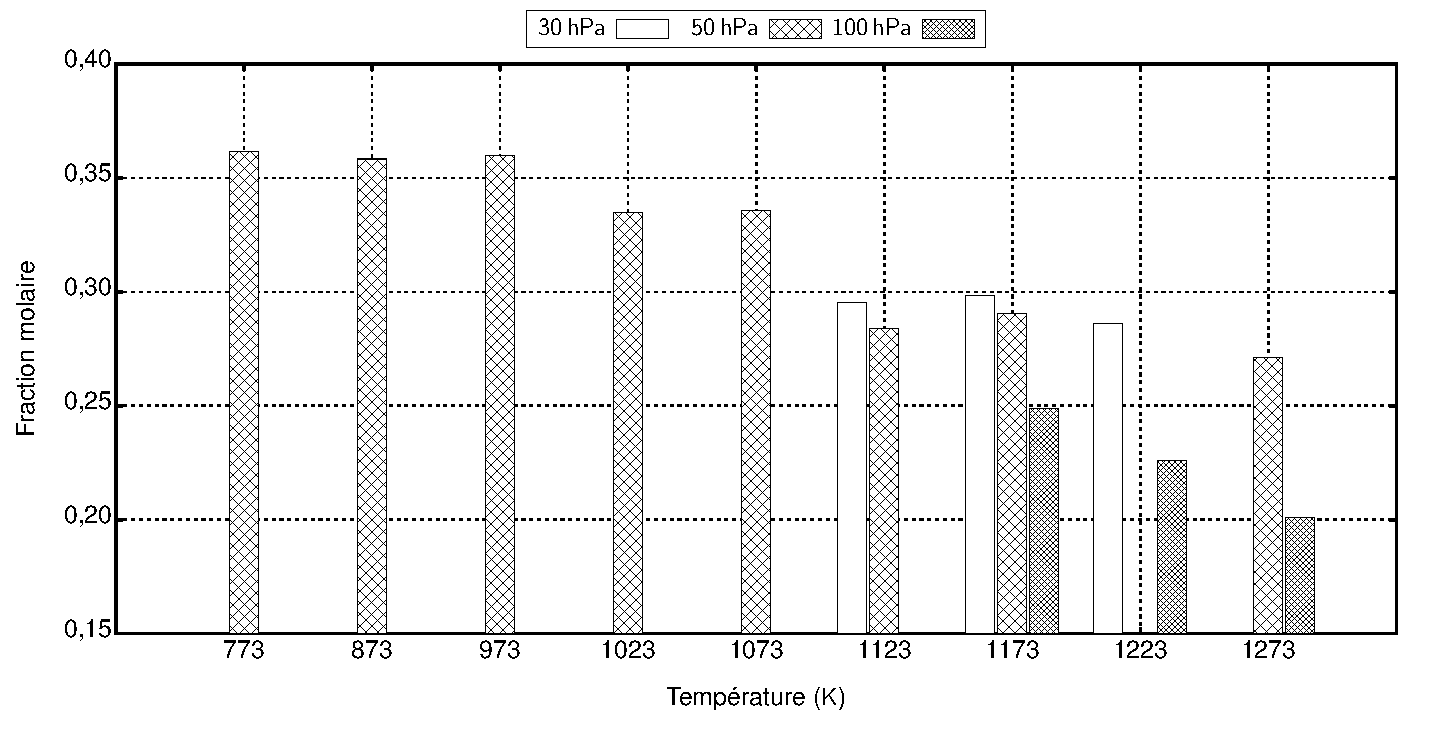
\includegraphics{figures/ch-03-decomposition_c2h2_bp}}
  }\\
  \subfloat[\label{fig:minoritaires_bp}Espèces minoritaires (qualitatif).]{
    \centering\resizebox{0.98\textwidth}{!}{
      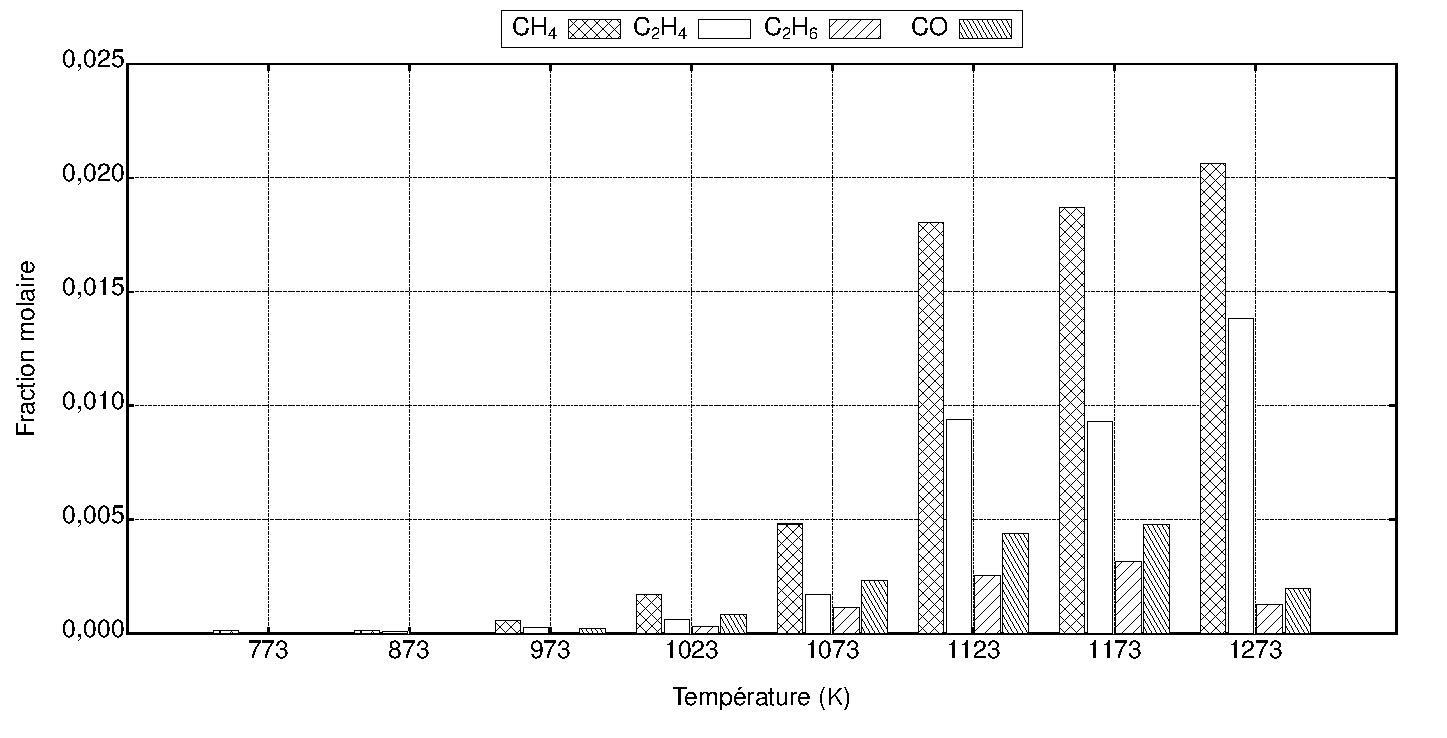
\includegraphics{figures/ch-03-reaction_byproducts_bp}}
  }

  \caption{\label{fig:pyrolyse_acetylene_bp}Pyrolyse du \ch{C2H2} à basse pression dans réacteur horizontal en quartz sous un débit total de \SI{222}{\sccm}: suivi \protect\subref{fig:acetylene_bp} de l'acétylène à la sortie en fonction de la température de contrôle et de la pression d'opération et \protect\subref{fig:minoritaires_bp} des espèces minoritaires à \SI{50}{\hecto\pascal}.}
\end{figure}

On observe Figure~\ref{fig:pyrolyse_acetylene_bp} qu'aucune décomposition du \ch{C2H2} n'a lieu jusqu'à une température de \SI{973}{\kelvin} pour les temps de séjour imposés par le débit total employé. La décomposition commence à devenir importante à partir de \SI{1123}{\kelvin}, température pour laquelle la fraction en acétylène à la sortie correspond à 86\% de celle injectée en entrée. On remarquera que cette valeur ne correspond pas exactement à une conversion de 14\% si l'on prend en compte le changement de volume molaire du gaz. Comme la décomposition ne peut pas être représentée par une réaction globale simple, comme cela est possible pour l'ammoniac, et que par ailleurs l'installation expérimentale utilisée ne comporte pas de système de mesure de débit en sortie, seule une estimation numérique, basée sur nos modèles, du taux de dissociation sera proposée. Les teneurs en \ch{CO} observées sont cohérentes avec la composition nominale de la bouteille \textendash{} le \ch{CO} est issu de l'acétone qui sert à stabiliser l'acétylène \textendash{} comme cela avait déjà été rapporté par \citet{Norinaga2005}. L'influence de la pression présentée Figure~\ref{fig:pyrolyse_acetylene_bp} s'avère être en accord avec la loi d'action de masse. Il faut préciser que la technique de prélèvement induit des difficultés posées par les variations \textendash{} augmentation \textendash{} de pression que l'on observe à \SI{30}{\hecto\pascal}, ce qui peut expliquer la proximité entre les résultats à \SIlist{30;50}{\hecto\pascal} Figure~\ref{fig:acetylene_bp}. Les fractions molaires en hydrocarbures fournies Figure~\ref{fig:minoritaires_bp} sont calculées à partir des intensités relatives des pics mesurés, aucun étalonnage n'étant réalisé~\footnote{Les intensités sont affectées à partir des diffusivités thermiques calculées~\cite{Lienhard2008}: l'estimation est faite en multipliant le facteur d'étalonnage de \ch{C2H2} par le rapport entre la diffusivité de l'espèce considérée et celle de l'acétylène. Le \ch{CO} a été étalonné normalement.}. Ces résultats seront comparés aux prédictions du modèle numérique présenté Chapitre~\ref{ch:modelisation_cinetique}.

\subsection{Cémentation à partir des hydrocarbures}
\label{sec:cementation-hydrocarbure}

La cémentation à partir des hydrocarbures présente quelques particularités par rapport à celle réalisée avec des mélanges \ch{CO-H2}. Les procédés qui utilisent \ch{C2H2} ou \ch{C2H4} comme source de carbone sont régis par la cinétique de catalyse de ces précurseurs et ses produits de décomposition homogène sur les surfaces traitées. La capacité de ces atmosphères de libérer des atomes de carbone est élevée, ce qui implique des potentiels carbone importants. En raison de la cinétique rapide des processus chimiques en phase gazeuse et hétérogènes, la mise au point de la cémentation à partir des hydrocarbures ne peut pas être traitée de la même façon que les procédés proches de l'équilibre, comme les atmosphères \ch{CO-H2}. \citet{Kula2005} ont montré l'importance relative des espèces constituant la couche d'espèces adsorbées formée en utilisant une atmosphère \ch{C2H2}/\ch{C2H4} dilué dans \ch{H2} sans qu'un dépôt carboné soit formé. Les auteurs~\cite{Kula2005} ont observé une faible concentration de radicaux \ch{C1}~\footnote{On notera \ch{C_{$n$}} l'ensemble de composés contenant $n$ atomes de carbone.} avec un maximum de concentration associé aux radicaux de la famille \ch{C2} suivi par une décroissance presque linéaire de l'importance des complexes adsorbés jusqu'à \ch{C7}, lesquels présentent une intensité très réduite. Ces résultats suggèrent l'importance des hydrocarbures légers dans la cémentation réalisée en pulses et donc l'intérêt d'éviter leur consommation dans l'atmosphère. Si l'enrichissement est réalisé avec un flux continu d'hydrocarbures, un dépôt carboné est normalement formé en surface. 
Bien que dans la pratique industrielle de la cémentation consiste en un enrichissement réalisé par pulses d'hydrocarbures pendant une durée de \SIrange{1}{5}{\minute}, en raison de notre installation expérimentale, nous avons tout de même choisi de réaliser des enrichissements en un flux continu. Cette pratique a un effet négligeable sur l'enrichissement de l'alliage en raison du dépôt carboné qui agit à haute température comme une source du carbone: des résultats similaires sont obtenus soit en imposant une condition contrôlée par la cinétique de surface soit en travaillant à concentration constante (dépôt carboné), ce qui permet de contrôler dans chaque cas l'enrichissement par le solide~\cite{Kula2005}. Une étude similaire réalisée par \citet{Gorockiewicz2010429} suggère que le dépôt carboné en surface est composé de graphite.

\subsubsection{Traitements à pression atmosphérique}

La dynamique d'enrichissement en carbone à partir des hydrocarbures à pression atmosphérique a été étudiée uniquement pour l'alliage 23MnCrMo5 à partir du suivi de prise de masse tout au long des traitements de cémentation. Ces traitements ont été réalisés à une température fixe de \SI{1173}{\kelvin} à la pression atmosphérique sous un débit total de \SI{500}{\sccm} dans des mélanges \ch{N2 - C2H2} contenant 0,5\% et 1,0\% d'acétylène en volume à l'entrée \textendash{} soit des pressions partielles d'environ \SI{5}{\hecto\pascal} et \SI{10}{\hecto\pascal}. Ces conditions sont résumées Tableau~\ref{tab:cementation-hydrocarbure}. Les échantillons ont été pesés avant et après traitement pour vérifier les résultats fournis par la thermobalance et permettre le calcul de la prise de masse par unité de surface. L'analyse par chromatographie en phase gazeuse des produits de pyrolyse \textendash{} et de décomposition hétérogène \textendash{} de l'acétylène a été réalisée pendant toute la durée des traitements.

\begin{table}[hb]
  \caption{\label{tab:cementation-hydrocarbure}Conditions de traitement pour la cémentation à pression atmosphérique (\SI{100}{\hecto\pascal}) à partir des mélanges \ch{N2 - $x$ C2H2}.}
  
  \centering{}\footnotesize{}
  \begin{tabular}{\$c^c^c^c}
    \toprule[2pt]
    \rowstyle{\bfseries}
    Température 
    & Débit 
    & Mélange 
    & Pression \ch{C2H2} 
    \tabularnewline
    \midrule[2pt]
    \multirow{2}{1cm}[-3pt]{\SI{1173}{\kelvin}} 
    & \multirow{2}{2cm}[-3pt]{\SI{500}{\sccm}} 
    & \ch{N2 - 0,010 C2H2} 
    & \SI{10}{\hecto\pascal}
    \tabularnewline[6pt]
    & 
    & \ch{N2 - 0,005 C2H2} 
    & \SI{5}{\hecto\pascal}
    \tabularnewline
    \bottomrule
  \end{tabular}
\end{table}

La Figure~\ref{fig:mass_intake_hydrocarbon} présente les prises de masse mesurées au cours des traitements et les simulations correspondantes réalisées en utilisant le coefficient de diffusion fourni par \citet{Slycke1981ii} pour des alliages du système \ch{Fe-C}. En raison de l'utilisation d'un volume de ballast pour homogénéiser le mélange gazeux avant son arrivée dans le réacteur, il a été nécessaire de décaler les courbes mesurées par thermogravimétrie pour que la prise de masse commence bien à l'instant $t=\SI{0}{\second}$. Ainsi, on élimine le délai correspondant à l'arrivée de l'acétylène dans la zone chaude du réacteur. Lors de l'arrivée du \ch{C2H2} l'enrichissement a apparemment lieu à flux constant pendant une durée comprise entre \SIlist{700;1000}{\second} environ, qui dépend de la concentration en entrée de ce précurseur et donc du chargement du ballast. La durée de cette période transitoire dans le régime d'enrichissement est de l'ordre de grandeur de celle observée par \citet{Kula2005} pour la formation d'une précipitation de carbures sur la nuance 20CrMnTi5-4-1.

\begin{figure}[h]
  \centering\resizebox{0.6\textwidth}{!}{
  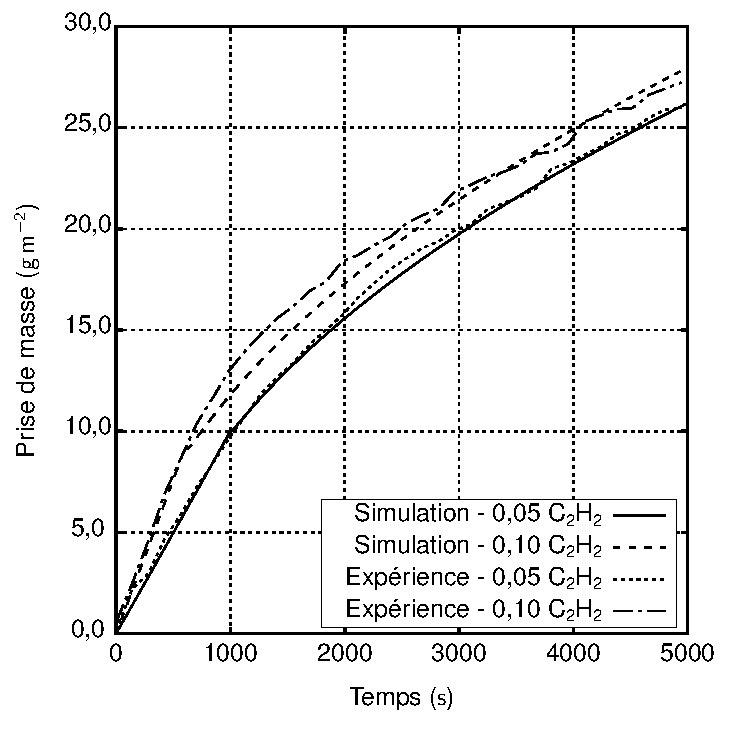
\includegraphics{figures/ch-03-mass_intake_hydrocarbon}}
  
  \caption{\label{fig:mass_intake_hydrocarbon}Comparaison des prises de masse en carbone à partir des hydrocarbures avec des simulations de l'équation de diffusion en utilisant le coefficient de diffusion fourni par \citet{Slycke1981ii} pour des alliages \ch{Fe-C} contenant des fractions en carbone équivalentes à la nuance 23MnCrMo5.}
\end{figure}

Pour ajuster les données nécessaires au modèle de diffusion, il faut supposer pendant cette période transitoire un flux en surface $J=\SI{5,6e-3}{\micro\mole\per\square\metre\per\second}$ pour 0,5\% de \ch{C2H2} à l'entrée ($J=\SI{8,5e-3}{\micro\mole\per\square\metre\per\second}$ pour 1,0\% de \ch{C2H2}). Pour satisfaire le comportement cinétique observé, selon la loi d'action de masse, il est normal que l'atmosphère contenant 0,5\% de \ch{C2H2} au départ produise un flux supérieur de 50\% à celui de l'atmosphère avec 1,0\% de \ch{C2H2} à l'entrée \textemdash{} celle plus riche en \ch{C2H2} ayant un avancement de décomposition homogène proportionnellement plus important. %Ces flux sont supérieurs à ceux produits par les taux de réaction proposés par \citet{Yada2013}, ce qui est lié au fait qu'il s'agit d'un alliage dont la diffusion a lieu en domaine multi-phasé et où la formation de cémentite ne représente pas la limite maximale d'enrichissement. 
Finalement une condition aux limites contrôlée par le transport en phase gazeuse s'établit, pour laquelle on calcule une constante de transfert de matière~\cite{Dulcy2007} $h\sim$~\SIlist{3;10}{\micro\mole\per\square\metre\per\second} correspondant aux deux atmosphères et une concentration en surface de l'ordre de 1,25-1,30\% en poids. Cette condition nécessaire pour expliquer les prises de masse mesurées implique la précipitation de cémentite pendant ces phases d'enrichissements. Le Tableau~\ref{tab:conditions-limite-pa} rassemble les expressions des flux utilisées dans les simulations des prises de masse pendant la période transitoire (flux constant) et à flux variable. Des pressions partielles de \ch{C2H2} de l'ordre de \SI{3}{\hecto\pascal} correspondant aux fractions en acétylène mesurées à la sortie du réacteur, lesquelles sont largement en dessous de celles à l'entrée, conduisent déjà à une condition de saturation en carbone à la surface des échantillons traités. %Selon \citet{Yada2013}, des pressions de l'ordre de 10\% de cette valeur seraient déjà suffisantes.

\begin{table}[h]
  \caption{\label{tab:conditions-limite-pa}Conditions aux limites pour la simulation de la prise de masse lors de la cémentation à pression atmosphérique. $C_{s}$ désigne la fraction molaire de carbone en surface.}
  
  \footnotesize{}\centering{}
  \begin{tabular}{\$l^l^l}
    \toprule[2pt]
    \multicolumn{1}{c}{\bfseries Type de condition}
    & \multicolumn{1}{c}{\bfseries 0,5\%~\ch{C2H2}}
    & \multicolumn{1}{c}{\bfseries 1,0\%~\ch{C2H2}}
    \tabularnewline
    \midrule[2pt]
    Flux constant 
    & $J=\SI{5,6e-3}{\micro\mole\per\square\metre\per\second}$ 
    & $J=\SI{8,5e-3}{\micro\mole\per\square\metre\per\second}$
    \tabularnewline
    Flux variable 
    & $J={3}\times(0,056-C_{s})~\si{\micro\mole\per\square\metre\per\second}$ 
    & $J={10}\times(0,057-C_{s})~\si{\micro\mole\per\square\metre\per\second}$
    \tabularnewline
    \bottomrule
  \end{tabular}
\end{table}

\subsubsection{Traitements à basse pression}

La cémentation de l'alliage 16NiCrMo13 a été réalisée sous une pression totale de \SI{50}{\hecto\pascal} à une température de \SI{1173}{\kelvin} avec les atmosphères et durées fournies Tableau~\ref{tab:cementation_bp}. Des débits de l'ordre de 2-3 fois supérieurs à ceux employés dans les études de pyrolyse ont pour but d'empêcher la décomposition homogène de \ch{C2H2} et donc de permettre l'arrivée du précurseur jusqu'à l'échantillon. Le résultat obtenu pour une atmosphère avec une pression partielle en \ch{C2H2} égale à \SI{2,5}{\hecto\pascal} suggère que la saturation en surface n'a pas été atteinte, ce qui se démarque des résultats à la pression atmosphérique si l'on considère que la pression partielle de \SI{3}{\hecto\pascal} mesurée dans les expériences à pression atmosphérique en sortie est responsable de l'enrichissement. Ceci n'est pas tout-à-fait vrai du fait de la décomposition de l'acétylène après contact avec l'échantillon. L'atmosphère carburante possède une pression partielle au moins supérieure à cette valeur à l'endroit où se trouve l'échantillon. Cela peut aussi être lié à la formation d'un dépôt carboné à pression atmosphérique \textendash{} observé sur les échantillons traités \textendash{} et à un contrôle cinétique à basse pression ne permettant pas d'atteindre la saturation en surface par des espèces carbonées.

\begin{table}[h]
  \caption{\label{tab:cementation_bp}Cémentation basse pression de l'alliage 16NiCrMo13.}
  
  \centering\footnotesize{}%
  \begin{tabular}{\$c^c^c^c^c^c}
    \toprule[2pt]
    \rowstyle{\bfseries}
    Atmosphère 
    & Débit 
    & Pression \ch{C2H2} 
    & Durée 
    & Surface traitée 
    & Gain de masse
    \tabularnewline
    \midrule[2pt]
    %
    \ch{N2 - 0,05 C2H2} 
    & \SI{636}{\sccm} 
    & \SI{2,5}{\hecto\pascal} 
    & \SI{3}{\hour} 
    & $8,80\times10^{-4}\,$\si{\square\metre} 
    & \SI{11,3}{\gram\per\square\metre}
    \tabularnewline
    %
    \ch{N2 - 0,25 C2H2} 
    & \SI{400}{\sccm} 
    & \SI{12,5}{\hecto\pascal} 
    & \SI{2}{\hour} & $8,80\times10^{-4}\,$\si{\square\metre} 
    & \SI{43,8}{\gram\per\square\metre}
    \tabularnewline
    \bottomrule
  \end{tabular}
\end{table}

Si l'on augmente la pression partielle de \ch{C2H2} à \SI{12,5}{\hecto\pascal} tout en réduisant le débit total à \SI{400}{\sccm}, la saturation en carbone à la surface est à nouveau atteinte et un fort enrichissement est observé. Ce résultat peut indiquer que la réaction de cémentation est composée \begin{inparaenum}[(i)] \item d'une réaction de craquage de \ch{C2H2} avec production de radicaux, ce qui peut se produire en surface comme dans le gaz et \item d'un apport de matière au solide. \end{inparaenum} En augmentant le débit, on limite la ré-absorption des radicaux et donc on reduit la réaction de cémentation. Alternativement, on peut supposer que le débit plus élevé empêche la formation d'un dépôt carboné pouvant assurer un enrichissement à concentration constante, ce qui représenterait une autre explication hydrodynamique au phénomène observé.

\section{Procédés utilisant de l'ammoniac}
\label{sec:pyrolyse_ammonia}

Les nitrurations gazeuses réalisées dans cette étude ont lieu sous des atmosphères à base d'ammoniac comme cela est présenté Tableau~\ref{tab:treatment_atmospheres} pour les traitements à la pression atmosphérique. Comme \ch{NH3} est très instable à \SI{1173}{\kelvin} \textendash{} température choisie pour les enrichissements \textendash{} l'équilibre entre la fraction résiduelle d'ammoniac à cette température et l'azote dans le matériau est utilisé pour le contrôle de l'atmosphère.  Thermo-Calc~\cite{Andersson2002,Borgenstam2000} permet de relier l'activité de l'azote dans le matériau à celle dans le gaz, permettant ainsi de généraliser la définition de potentiel nitrurant. La mise au point de l'atmosphère pour la nitruration se fait donc à partir des mesures de l'ammoniac résiduel dans le réacteur non-chargé et du calcul du potentiel de nitruration $K_{N}$ pour chaque alliage \textemdash{} voir Annexe~\ref{an:nitriding-kn}.

\subsection{Décomposition à la pression atmosphérique}

Le suivi de la décomposition de l'ammoniac à pression atmosphérique a été réalisé dans la plage de températures comprises entre \SIlist{773;1223}{\kelvin} en utilisant la chromatographie en phase gazeuse \textendash{} détecteur du type TCD \textendash{} pour la mesure de l'ammoniac résiduel. Les conditions expérimentales sont résumées Tableau~\ref{tab:decomposition-conditions-pa}.

\begin{table}[h]
  \caption{\label{tab:decomposition-conditions-pa}Conditions expérimentales pour l'étude de la décomposition de \ch{NH3} à pression atmosphérique dans le réacteur présenté Figure~\ref{fig:reacteur_pa}.}
  
  \footnotesize{}\centering{}
  \begin{tabular}{\$c^c^c^c^c}
    \toprule[2pt]
    \rowstyle{\bfseries}
    Température 
    & Débit 
    & Mélange 
    & Pression totale 
    & Pression \ch{NH3}
    \tabularnewline
    \midrule[2pt]
    \SIrange{773}{1223}{\kelvin}
    & \SI{415}{\sccm}
    & \ch{0,24 N2 - 0,72 H2 - 0,04 NH3}
    & \SI{1000}{\hecto\pascal}
    & \SI{40}{\hecto\pascal}
    \tabularnewline
    \bottomrule
  \end{tabular}
\end{table}

Les résultats (Figure~\ref{fig:ammonia_decomposition}) du suivi de la décomposition de l'ammoniac à la pression atmosphérique dans le réacteur en alumine décrit Section~\ref{sec:experimental_system} montrent un palier de conversion de l'ammoniac en dessous de \SI{900}{\kelvin} avec un taux de conversion $\alpha$ de l'ordre de 10\%. La faible vitesse de décomposition de l'ammoniac est connue depuis longtemps~\cite{Christiansen1935} et même en considérant l'effet de décomposition hétérogène sur les parois d'un réacteur en quartz~\cite{Cooper1988,Dirtu2006}, l'avancement de la réaction n'est pas très rapide. C'est à partir de ce comportement qu'un contrôle à l'état stationnaire du procédé est possible, donc à partir du débit~\cite{Gantois2010}. Lorsque l'atmosphère (Tableau~\ref{tab:treatment_atmospheres}) est composée d'un mélange ammoniac/ammoniac-craqué, le taux de conversion $\alpha$ de l'ammoniac doit être calculé en tenant compte du changement de volume apporté par la réaction globale de décomposition \ch{NH3 <=> 1/2 N2 + 3/2 H2}. La procédure généralisée présentée dans l'Annexe~\ref{an:ammonia_decomposition} est utilisée.

À partir de ce palier à \SI{900}{\kelvin}, \ch{NH3} devient très instable et la conversion augmente rapidement avec la température de la zone chaude du réacteur, pour atteindre 90\% à une température de \SI{1223}{\kelvin}. À \SI{1173}{\kelvin}, température adoptée pour les traitements thermochimiques dans ce travail, une fraction molaire résiduelle d'ammoniac égale à $5,5\times10^{-3}$ a été mesurée pour les conditions opératoires décrites. Après correction de la fraction molaire en dihydrogène issu de l'ammoniac décomposé, on trouve un potentiel nitrurant $K_{N}=\SI{8,6e-03}{\atm^{-0,5}}$.  D'après les diagrammes présentés Figure~\ref{fig:diagrammes_kn}, le traitement devrait produire des fractions massiques en azote atomique sur les surfaces traitées de l'ordre de 0,009 pour l'alliage 16NiCrMo13 et 0,010 pour la nuance 23MnCrMo5. Des résistances de transfert de matière à l'interface, liées à la composition des nuances traitées, peuvent limiter l'enrichissement.  Physiquement, ceci est lié au fait que les surfaces métalliques traitées catalysent le craquage du précurseur de nitruration et donc seule une faible fraction des molécules de \ch{NH3} adsorbées sur le métal apporte effectivement~\cite{Wrobel2006,Arabczyk2009} de l'azote à l'alliage. Dans le cas plus général des réacteurs industriels, les structures constituant le four sont à considérer.

\subsection{Décomposition sous pression réduite}
\label{sec:decomposition_nh3_bp}

Aux températures employées dans les traitements en phase austénitique des matériaux, l'ammoniac devrait être presque complètement dissocié. Ceci a été mis en évidence à la pression atmosphérique. Ce n'est toutefois pas le cas à basse pression pour des débits similaires. Cela est le résultat de l'augmentation de la vitesse moyenne du gaz qui évolue à l'inverse de la pression de travail. En utilisant une atmosphère composée de \ch{N2 - 0,25 NH3} à \SI{50}{\hecto\pascal} sous un débit total de \SI{684}{\sccm} aucune décomposition mesurable n'est observée dans la zone chaude du réacteur \textemdash{} de \SIrange{473}{1173}{\kelvin}.  Pour vérifier comment agit la loi d'action de masse, nous avons utilisé une atmosphère \ch{N2 - 0,64 NH3} sous un débit \SI{737}{\sccm} une fois à une pression de \SI{50}{\hecto\pascal} et à \SI{1173}{\kelvin} et une fois à une pression de \SI{100}{\hecto\pascal} et à \SI{1223}{\kelvin}. Aucune décomposition n'a été détectée et ces conditions ont été choisies pour la nitruration. Le Tableau~\ref{tab:decomposition-conditions-bp} rassemble ces conditions. 

\begin{table}[!h]
  \caption{\label{tab:decomposition-conditions-bp}Conditions expérimentales pour l'étude de la décomposition du \ch{NH3} à basse pression dans le réacteur présenté Figure~\ref{fig:reacteur_bp}.}
  
  \footnotesize{}\centering{}
  \begin{tabular}{\$c^c^c^c^c}
    \toprule[2pt]
    \rowstyle{\bfseries}
    Température 
    & Débit 
    & Mélange 
    & Pression totale 
    & Pression \ch{NH3}
    \tabularnewline
    \midrule[2pt]
    \SIrange{473}{1173}{\kelvin}
    & \SI{684}{\sccm}
    & \ch{0,75 N2 - 0,25 NH3}
    & \SI{50}{\hecto\pascal}
    & \SI{12,5}{\hecto\pascal}
    \tabularnewline
    %
    \SI{1173}{\kelvin}
    & \SI{737}{\sccm}
    & \ch{0,36 N2 - 0,64 NH3}
    & \SIlist{50;100}{\hecto\pascal}
    & \SIlist{32;64}{\hecto\pascal}    
    \tabularnewline
    %
    \SIrange{773}{1173}{\kelvin}
    & \SI{470}{\sccm}
    & \ch{NH3}
    & \SIlist{50;100}{\hecto\pascal}
    & \SIlist{50;100}{\hecto\pascal}         
    \tabularnewline  
    \bottomrule
  \end{tabular}
\end{table}

En réduisant le débit à \SI{470}{\sccm} et en utilisant une atmosphère composée d'ammoniac pur, on mesure un faible taux de décomposition qui conduit à la formation d'une fraction de moins de 0,04 en diazote. Cette décomposition est liée au temps de séjour plus important dans la zone chaude du réacteur et est légèrement plus prononcée à \SI{100}{\hecto\pascal} qu'à \SI{50}{\hecto\pascal}, comme attendu.  La Figure~\ref{fig:ammoniac_bp} présente l'ammoniac résiduel en fonction de la température de la zone chaude du réacteur. La fin du palier de stabilité de l'ammoniac est cohérent avec les résultats à la pression atmosphérique (Figure~\ref{fig:ammonia_decomposition}). Seul l'ammoniac et le diazote ont été séparés par les colonnes du chromatographe.

\begin{figure}[h]
  \centering
  \subfloat[\label{fig:ammonia_decomposition}Pression atmosphérique.]{
    \centering\resizebox{0.98\textwidth}{!}{
    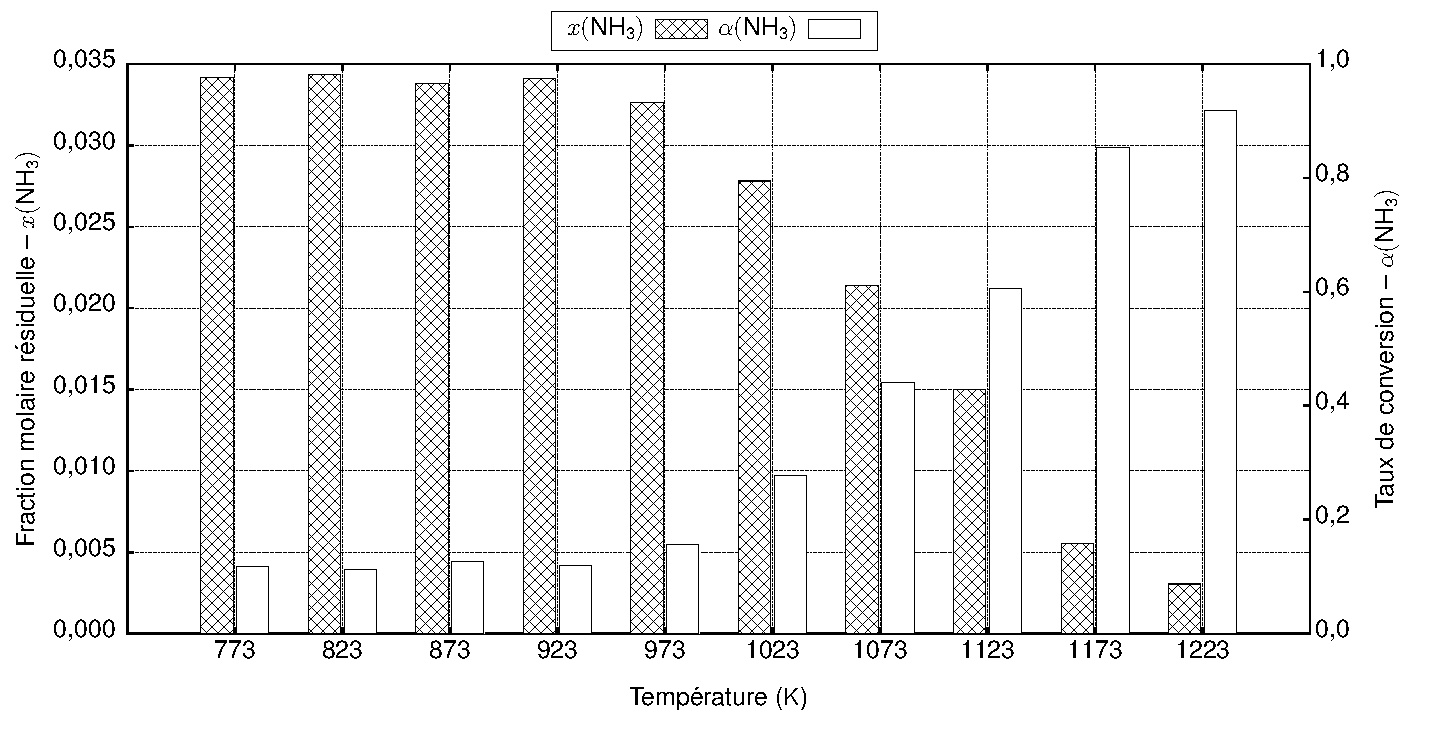
\includegraphics{figures/ch-03-decomposition_nh3_pa}}
  }\\
  \subfloat[\label{fig:ammoniac_bp}Basse pression.]{
    \centering\resizebox{0.98\textwidth}{!}{
    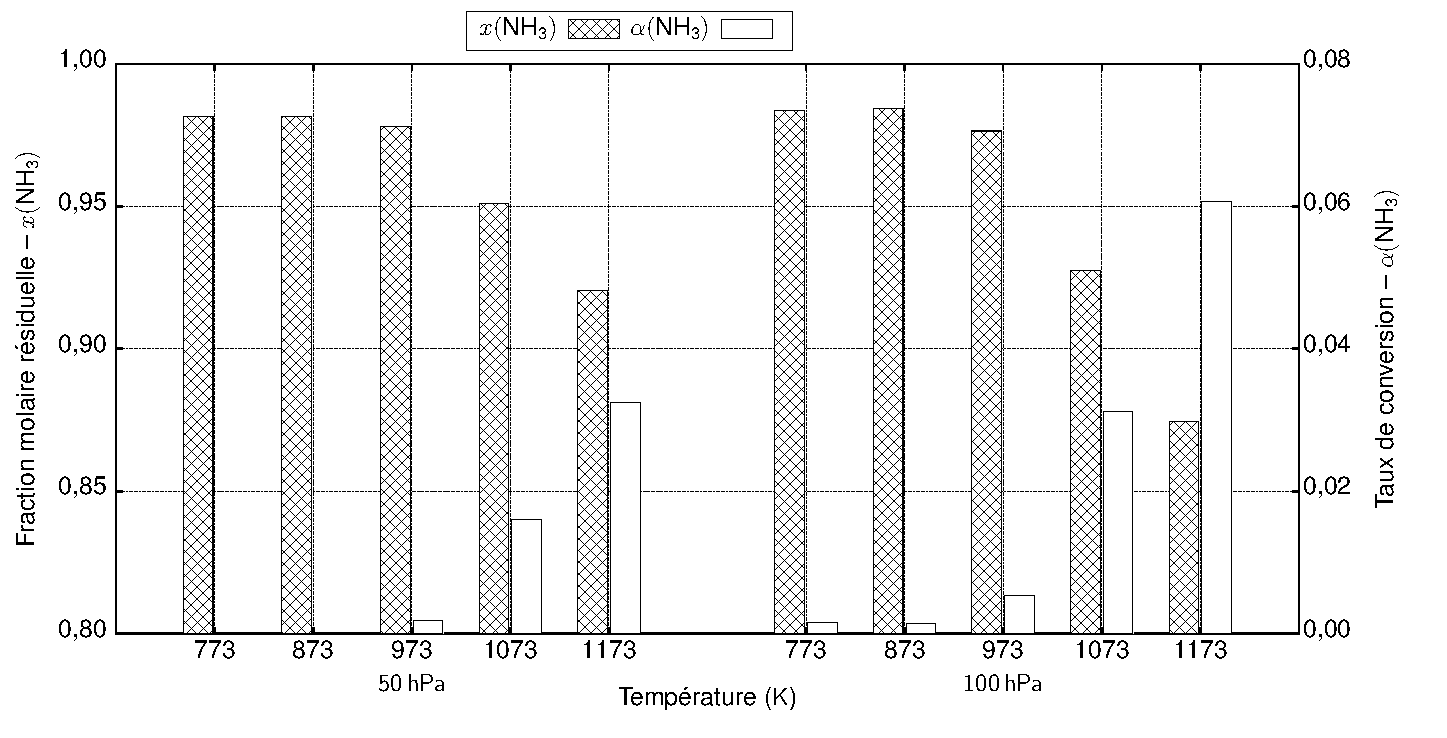
\includegraphics{figures/ch-03-decomposition_nh3_bp}}
  }

  \caption{\label{fig:ammoniac_residuel}Ammoniac résiduel et taux de conversion en fonction de la température de la zone chaude du réacteur: résultats \protect\subref{fig:ammonia_decomposition} à pression atmosphérique et \protect\subref{fig:ammoniac_bp} basse pression.}
\end{figure}

\subsection{Nitruration sous pression réduite}
\label{sec:nitruration-ammoniac}

La nitruration austénitique à basse pression de l'alliage 16NiCrMo13 a été conduite à \SI{1173}{\kelvin} sous une pression de \SI{50}{\hecto\pascal} pendant \SI{3}{\hour}. Ce traitement a été réalisé sous une atmosphère \ch{N2 - 0,64 NH3} avec un débit total de \SI{737}{\sccm} et sous une atmosphère \ch{N2 - 0,23 NH3} sous un débit total de \SI{682}{\sccm}.  Ces conditions ont été choisies en fonction des résultats de la Section~\ref{sec:decomposition_nh3_bp} où il a été montré qu'aucune décomposition de l'ammoniac n'est détectée dans la limite de précision de nos mesures. Le Tableau~\ref{tab:nitruration_bp} présente les traitements réalisés avec les surfaces métalliques exposées et les gains de masse respectifs des échantillons.

\begin{table}[h]
  \caption{\label{tab:nitruration_bp}Nitruration austénitique de l'alliage 16NiCrMo13.}
  
  \centering\footnotesize{}
  \begin{tabular}{\$c^c^c^c}
    \toprule[2pt]
    \rowstyle{\bfseries}
    Atmosphère 
    & Débit 
    & Surface traitée 
    & Gain de masse
    \tabularnewline
    \midrule[2pt] 
    \multirow{2}{*}{\ch{N2 - 0,64 NH3}} 
    & \multirow{2}{*}{\SI{737}{\sccm}} 
    & \SI{1,81e-3}{\square\metre} 
    & \SI{13,1}{\gram\per\square\metre}
    \tabularnewline
    %\cmidrule{3-4} 
    &  
    & \SI{9,54e-4}{\square\metre} 
    & \SI{18,5}{\gram\per\square\metre}
    \tabularnewline
    %
    \ch{N2 - 0,23 NH3} 
    & \SI{682}{\sccm} 
    & \SI{8,80e-4}{\square\metre} 
    & \SI{9,3}{\gram\per\square\metre}
    \tabularnewline
    \bottomrule
  \end{tabular}
\end{table}

On observe un gain de masse par unité de surface plus important pour la condition la plus riche en ammoniac.  En revanche, l'atmosphère contenant une fraction en ammoniac de 0,64 conduit à un enrichissement plus important si le réacteur est moins chargé. Le chargement de \SI{1,81e-3}{\square\metre} correspond à deux échantillons de dimensions équivalentes de \SI{9,54e-4}{\square\metre} placés côté-à-côté dans la même section transversale du réacteur: le taux de craquage en surface est plus prononcé dans la condition où la surface exposée est plus importante \textemdash{} le nombre de moles du système augmente plus rapidement, ce qui entraîne une accélération plus prononcée du mélange et donc un temps de séjour plus court. L'enrichissement est donc moins prononcé, même si l'atmosphère de départ est constante et que le flux de \ch{NH3} en phase gazeuse est largement supérieur à celui requis pour enrichir le solide. En raison de cette hétérogénéité, l'obtention d'une constante cinétique ne peut pas être directe. 

La Figure~\ref{fig:bilan_matiere_nitruration_bp} présente le bilan des espèces mesurées par chromatographie gazeuse pendant les traitements. On vérifie que les fractions en \ch{NH3} en sortie à l'état stationnaire \textendash{} fin de traitement \textendash{} pour l'atmosphère \ch{N2 - 0,64 NH3} sont indépendantes de la surface exposée. Ce n'est possible que si l'hypothèse de changement de temps de séjour \textendash{} ici il vaudrait mieux parler de \og{}temps de contact\fg{} \textendash{} proposée pour expliquer l'enrichissement est valable, ou que \ch{NH3} est formé après contact avec l'échantillon par récombinaison de ses produits de déshydrogénation partielle, via des processus du type \ch{NH + H <=> NH2} et \ch{NH2 + H <=> NH3}. 

Il faut aussi remarquer sur la Figure~\ref{fig:bilan_matiere_nitruration_bp} que la pente de la fraction molaire de \ch{NH3} au cours du traitement est plus élevée pour la condition la moins chargée (surface exposée moins importante), ce qui indique l'établissement d'un état stationnaire plus rapide et confirme les observations précédentes. Cela implique que pour des applications industrielles à basse pression, le diagnostic de la phase gazeuse pour la mise au point de traitements dépendra du chargement \textendash{} et naturellement de l'état de surface des pièces \textendash{} ainsi que du débit et donc pas seulement de l'ammoniac résiduel en équilibre avec les surfaces. Ce n'est qu'après l'établissement de l'état stationnaire qu'une condition aux limites de type concentration constante est possible. De cette manière l'enrichissement se fait globalement avec une condition transitoire sur les surfaces.

\vfill
\begin{figure}[!ht]
  \centering\noindent
  \begin{tikzpicture}
   \node at (0.0,+0.0) {
     \centering\noindent
     \begin{tikzpicture}%
     \node[anchor=south west,inner sep=0] (A) at (0,0) {%
       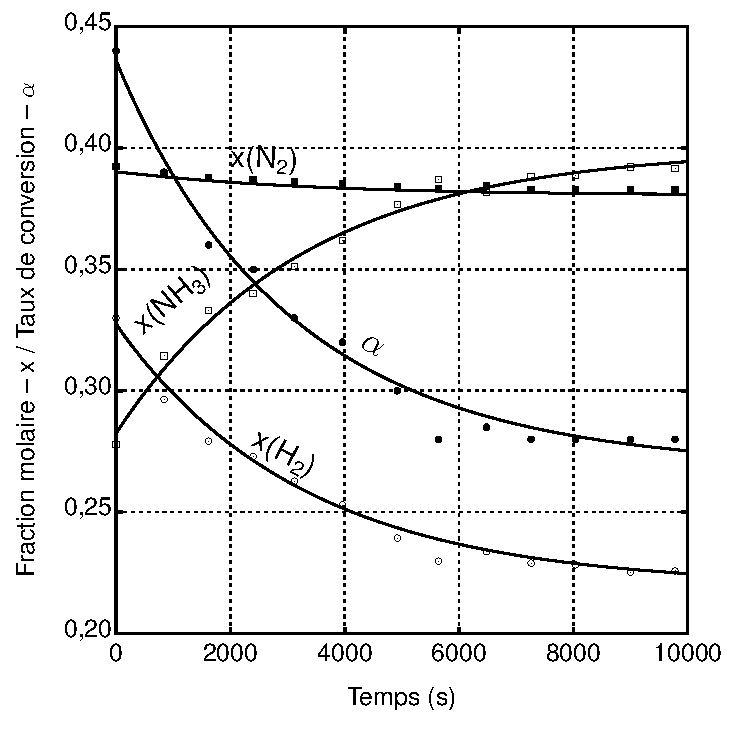
\includegraphics[width=7.5cm]
       {figures/ch-03-nitriding_balance_bp_experiment_1}
     };
     \begin{scope}[x={(A.south east)},y={(A.north west)}]
       \node at (0.55,1.0) 
       {\footnotesize\ch{N2 - 0,64 NH3} - S~=~\SI{1,81e-3}{\square\metre}};
     \end{scope}
     \end{tikzpicture}
   };
   \node at (8.0,+0.0) {
     \centering\noindent
      \begin{tikzpicture}%
      \node[anchor=south west,inner sep=0] (A) at (0,0) {%
        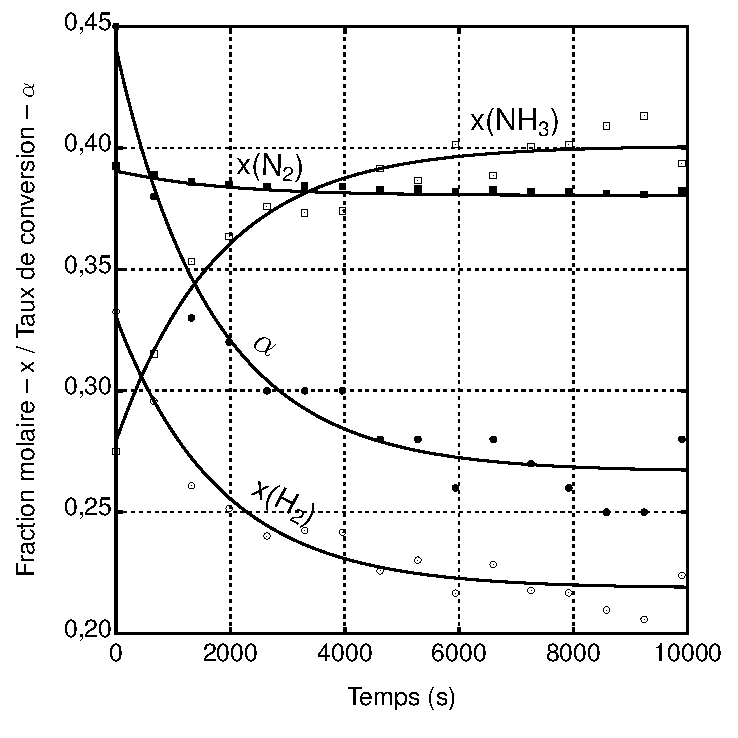
\includegraphics[width=7.5cm]
        {figures/ch-03-nitriding_balance_bp_experiment_2}
      };
      \begin{scope}[x={(A.south east)},y={(A.north west)}]
      \node at (0.55,1.0) 
      {\footnotesize\ch{N2 - 0,64 NH3} - S~=~\SI{9,54e-4}{\square\metre}};
      \end{scope}
      \end{tikzpicture}
   };
   \node at (4.0,-8.0) {
     \centering\noindent
      \begin{tikzpicture}%
      \node[anchor=south west,inner sep=0] (A) at (0,0) {%
        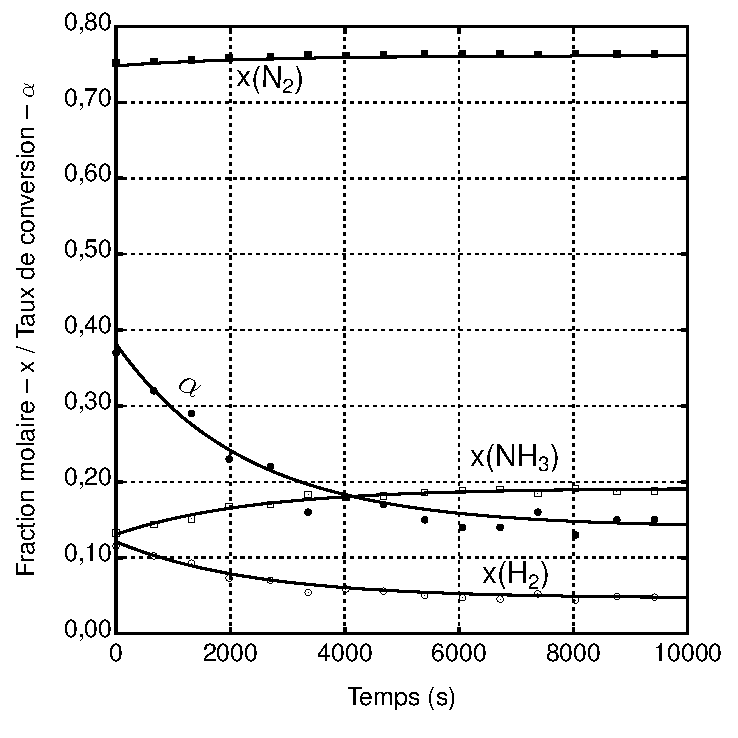
\includegraphics[width=7.5cm]
        {figures/ch-03-nitriding_balance_bp_experiment_3}
      };
      \begin{scope}[x={(A.south east)},y={(A.north west)}]
      \node at (0.55,1.0) 
      {\footnotesize\ch{N2 - 0,23 NH3} - S~=~\SI{8,80e-4}{\square\metre}};
      \end{scope}
      \end{tikzpicture}
   };
  \end{tikzpicture}

  \caption{\label{fig:bilan_matiere_nitruration_bp}Bilan matière de la nitruration austénitique: évolution des fractions molaires des espèces à la sortie du réacteur pour les traitements réalisés en utilisant des atmosphères \ch{N2 - 0,64 NH3}. Les données pour \ch{NH3} et \ch{N2} sont issues des mesures, tandis que pour \ch{H2} elles ont été calculées.}
\end{figure}
\vfill

\clearpage\section{Conclusion}

Cette section concerne les résultats expérimentaux présentés Chapitre~\ref{ch:caracterisation_atmospheres} sur la mise au point des atmosphères utilisées dans les traitements thermochimiques. Ce chapitre peut se résumer ainsi:
\begin{itemize}
  \item les études ont été réalisées dans des réacteurs tubulaires à pression atmosphérique et à basse pression; le transport des espèces dans le réacteur à pression atmosphérique a été caractérisé en utilisant la méthode du pulse d'un traceur; un système d'échantillonnage à basse pression a été présenté pour les études de décomposition des précurseurs;
  
  \item la température de point de rosée de l'atmosphère employée pour la cémentation des alliages a été calculée en fonction de la teneur en carbone visée sur les surfaces; ces résultats se trouvent être en bon accord avec les méthodes classiques;
  
  \item la pyrolyse de l'acétylène a été étudiée à pression atmosphérique et à basse pression; dans les deux cas on a suivi les hydrocarbures de types $C_{1}$ et $C_{2}$; pour les temps de séjour mesurés du réacteur à pression atmosphérique, l'avancement de la réaction de pyrolyse dépasse les 75\% et le bilan matière montre que des espèces et radicaux fortement carbonés sont présents en sortie du réacteur; cependant, à basse pression, le taux de décomposition n'est que de 20\% à \SI{30}{\hecto\pascal} et de 60\% à \SI{100}{\hecto\pascal} à partir d'un mélange \ch{N2 - 0,36 C2H2};
  
  \item à partir de la décomposition de l'ammoniac à la pression atmosphérique on a établi la condition aux limites d'enrichissement pour les simulations de diffusion de l'azote dans le matériaux; contrairement à la thermodynamique de la réaction globale de décomposition de \ch{NH3}, de très faibles niveaux de conversion ont été mesurés à basse pression même à \SI{1173}{\kelvin}, ce qui a été attribué à l'effet cinétique d'action de masse dans le système;
  
  \item la cémentation à partir des hydrocarbures permet l'enrichissement même au--delà de la saturation en surface et les résultats suggèrent un mécanisme de craquage suivie d'une adsorption conduisant à l'enrichissement au lieu d'un enrichissement direct par craquage des hydrocarbures en surface;
  
  \item des résultats similaires ont été obtenus pour la nitruration en domaine austénitique. La variation de surface de la charge du réacteur, qui conduit à des résultats similaires en concentration à la sortie des produits formés permet d'inférer que la recombinaison des produits de décomposition conduit à reformer en partie \ch{NH3} en phase gazeuse. 
\end{itemize}

\endinput